\documentclass[12pt]{article}
\usepackage{parskip}
\usepackage[letterpaper, margin=1in]{geometry}
\usepackage{graphicx}
%\usepackage{svg}
\usepackage{amsmath}
\usepackage{enumitem}
\usepackage{caption}
\usepackage{subcaption}
\usepackage{gensymb}
\graphicspath{{./images/}}
\title{ELECENG 3EJ4 Lab 2}
\author{Raeed Hassan \\ hassam41 \\ McMaster University}
\begin{document}
\maketitle
\pagebreak
\begin{itemize}
    \section*{Part 1}
    % A) Prelab: ~1.1, ~1.2, 1.3
    % B) Prelab: ~1.4, ~1.5 (Vo1 = -3.82, Vo2 = -4.15), ~1.6, ~1.7
    % C) In-lab: 1.8, 1.9, 1.10, 1.11
    % D) In-lab: 1.12, 1.13, 1.14, 1.15, 1.16, 1.17, 1.18, 1.19
    \item [\textbf{Q1.}]
    The $V_{o,min}$ and $I_o$ of the current sink determined from the simulation data in Step 1.2 are $V_{o,min} = -3$ V and $I_o = 0.185$ mA. The simulation data is shown in Figure \ref{fig:Step1.2}. The $V_{o,min}$ and $I_o$ of the current sink determined from the measurement data were $V_{o,min} = -3$ V and $I_o = 0.199$ mA. The measurement data is shown in Figure \ref{fig:Step1.10}. The measured $V_{o,min}$ value was the same as the simulated value, and the measured $I_o$ value was similar to the simulated value.
    \begin{figure}[!ht]
        \centering
        \begin{subfigure}[b]{0.45\textwidth}
            \centering
            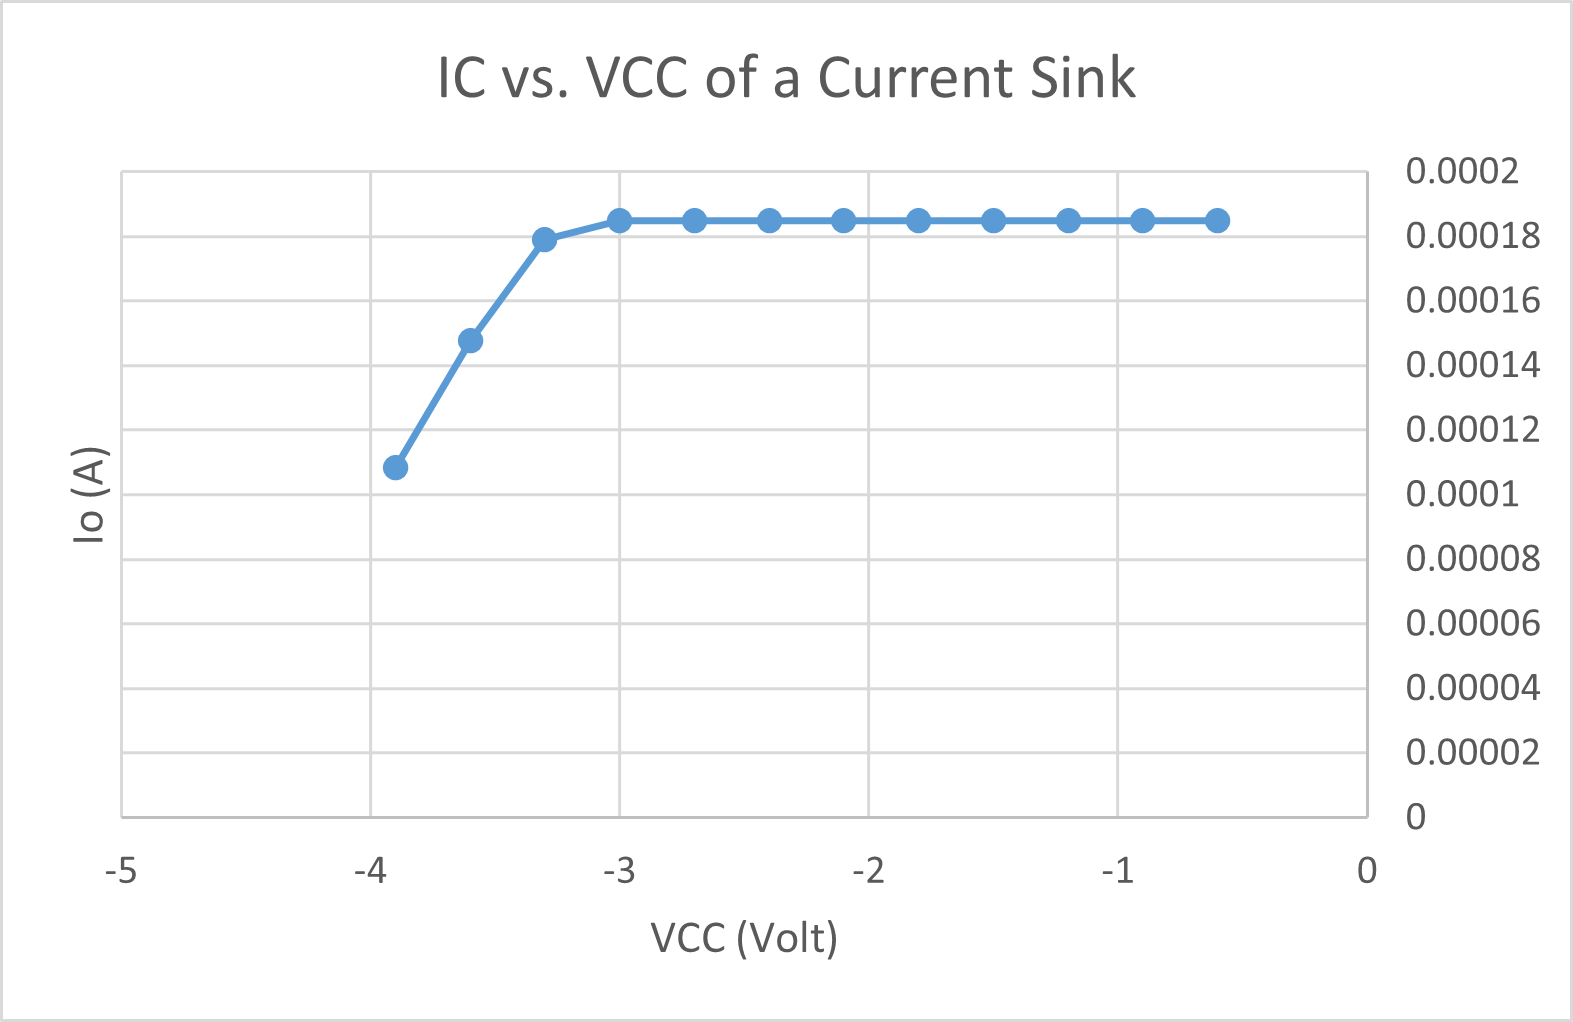
\includegraphics[width=\textwidth]{Step1.2}
            \caption{Step 1.2}
            \label{fig:Step1.2}
        \end{subfigure}
        \begin{subfigure}[b]{0.46\textwidth}
            \centering
            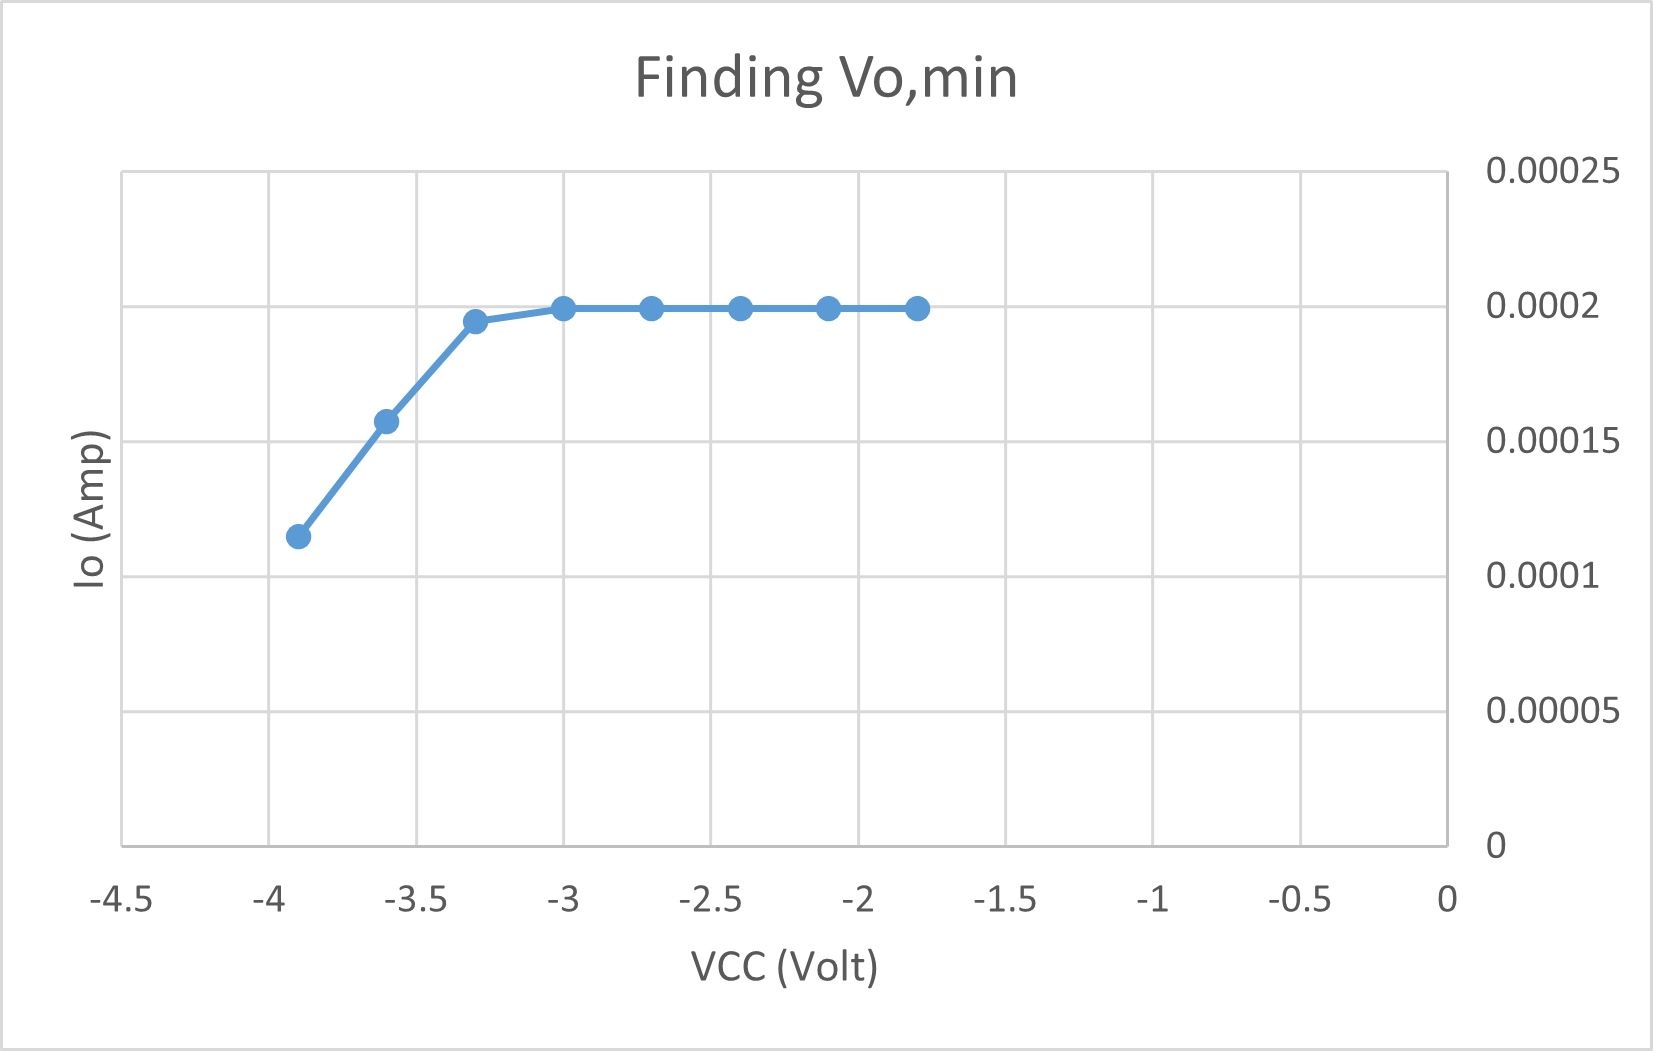
\includegraphics[width=\textwidth]{Step1.10}
            \caption{Step 1.10}
            \label{fig:Step1.10}
        \end{subfigure}
        \caption{Determination of $V_{o,min}$ and $I_o$ of current sink}
    \end{figure}
    \item [\textbf{Q2.}]
    The values determined in Step 1.5 were $V_{o1} = 4.94$ V and $V_{o2} = -3.58$ V. These values are close to the maximum and minimum output voltages due to the value of $V_{sig}$ at $V_{o1}$ and $V_{o2}$ being outside of the range the circuit works as an amplifier. 
    \item [\textbf{Q3.}]
    \begin{enumerate}
        \item The simulated DC $V_o$ vs $V_{sig}$ characteristics plot is shown in Figure \ref{fig:Step1.6}.
        \begin{figure}[!ht]
            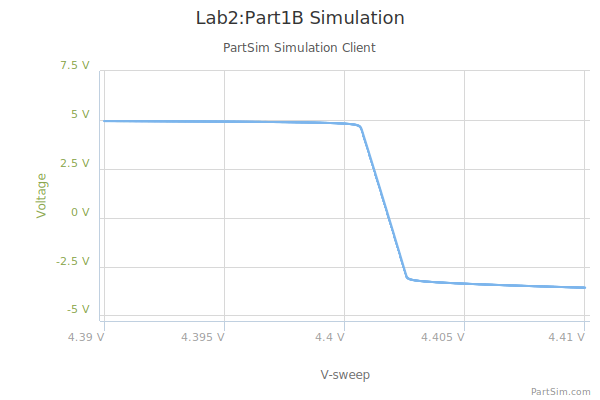
\includegraphics[width=\textwidth]{Step1.6}
            \caption{Simulated DC $V_o$ vs. $V_{sig}$ characteristics}
            \label{fig:Step1.6}
        \end{figure}
        \item For the circuit to work as an amplifier, the DC input range for $V_{sig}$ is between 4.4005 V and 4.4025 V and the output voltage range for $V_o$ is between 5 V and $-3.6$ V.
        \item The value of $V_{sig}$ for $V_o \approx 0$ V is $V_{sig} = 4.40183$ V, where the collector current $I_{C2} = 185$ $\mu$A.
        \item The measured DC $V_o$ vs $V_{sig}$ characteristics plot is shown in Figure \ref{fig:Step1.15}.
        \begin{figure}[!ht]
            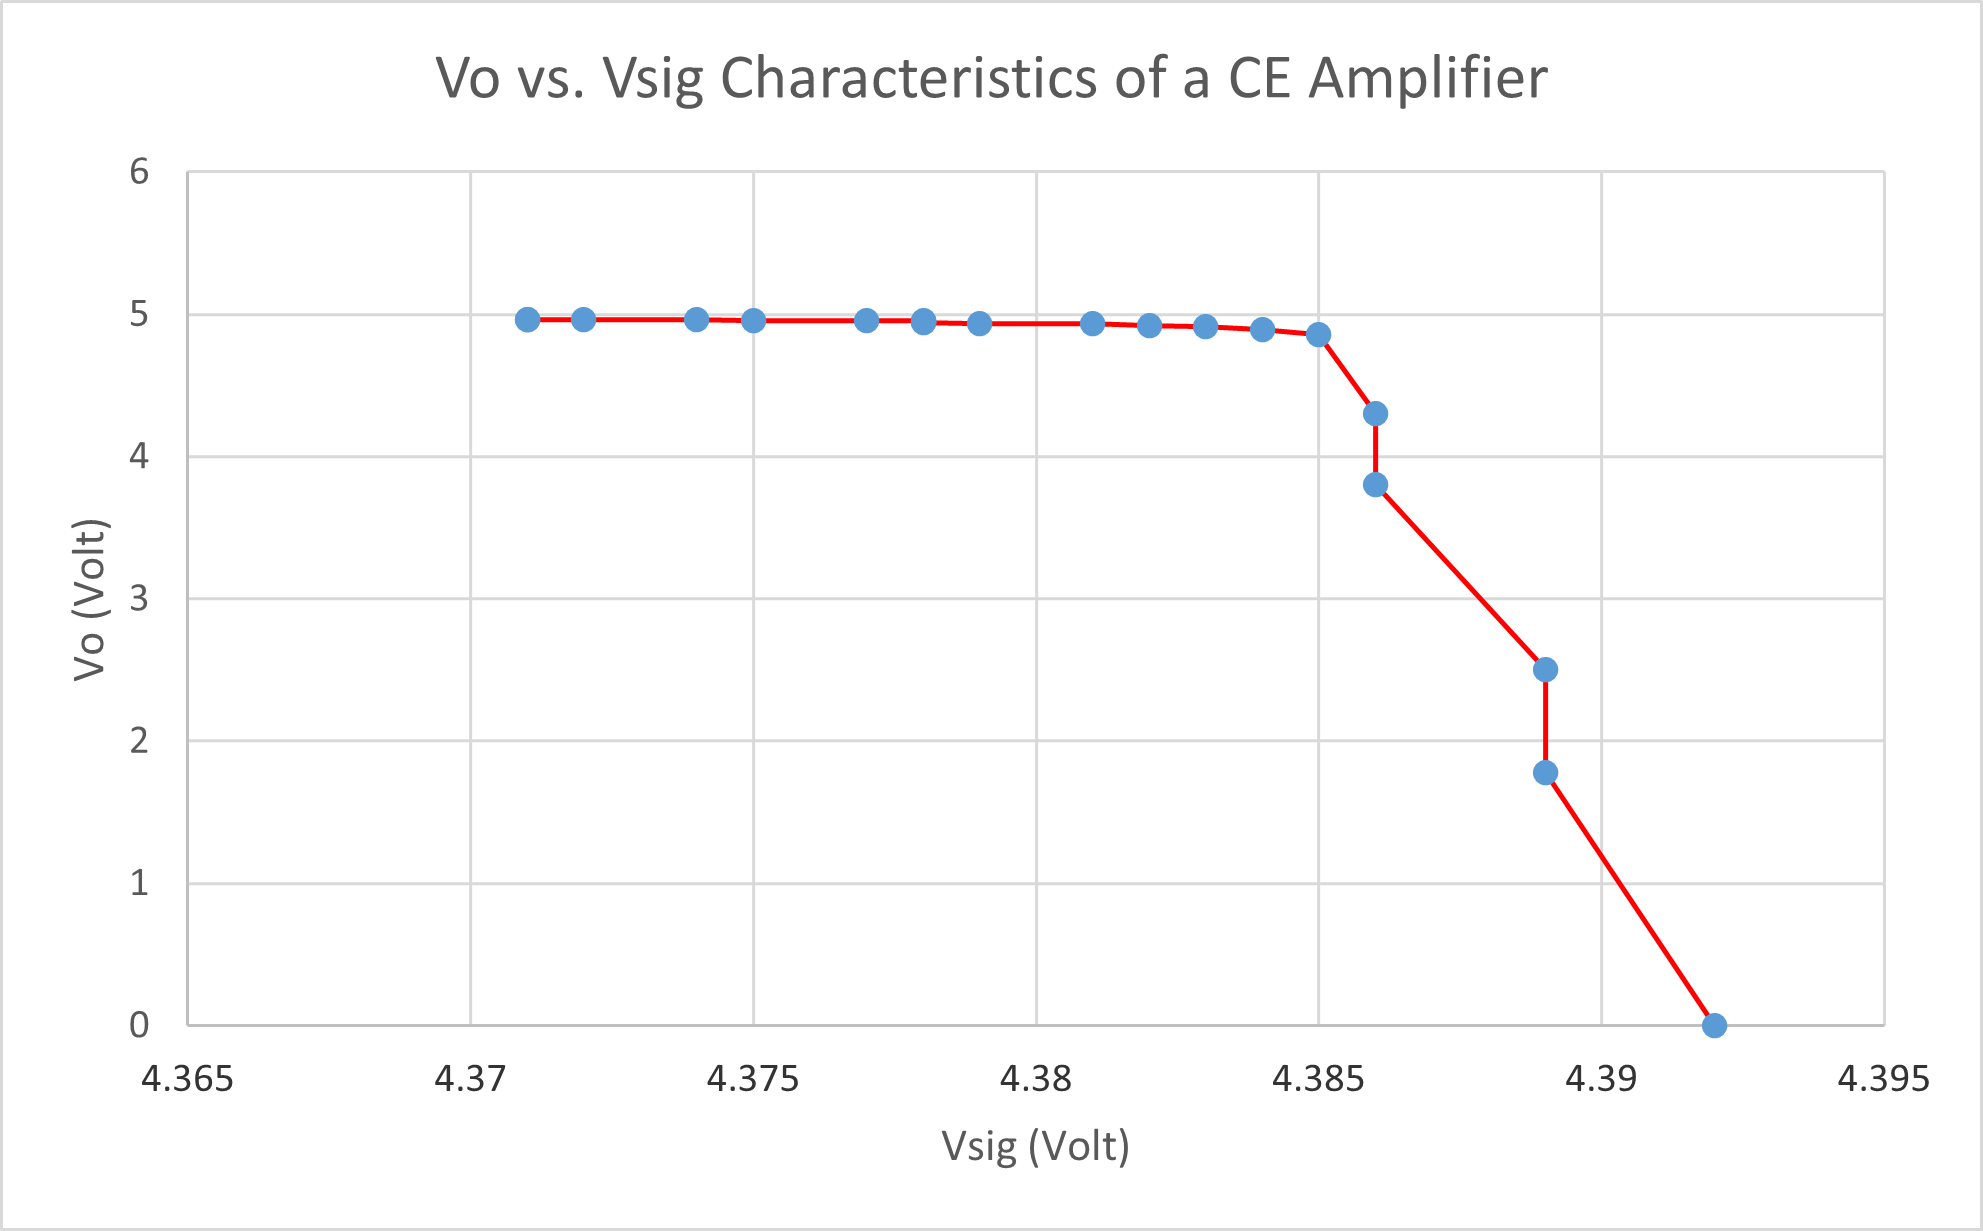
\includegraphics[width=\textwidth]{Step1.15}
            \caption{Measured DC $V_o$ vs. $V_{sig}$ characteristics}
            \label{fig:Step1.15}
        \end{figure}
    \end{enumerate}
    \item [\textbf{Q4.}]
    \begin{enumerate}
        \item The magnitude (in dB) and phase of the intrinsic voltage gain $A_{vo}$ at low frequency (100 Hz) are 12.15 dB and 180\degree. The upper 3-dB frequency is approximately 14.4 KHz. The bode plots (with real magnitude and phase in degrees) are shown in Figure \ref{fig:Step1.7}.
        \item The voltage gain $A_{vo}$ calculated using the measured data in Steps 1.17 and 1.18 was 63.4 dB.
        \item The value of $A_{vo}$ was 62.9 dB, very similar to the gain calculated at 100 Hz. However, the amplitudes of both signals were close to 0.707 of their original values ($V_{QB2} = 0.7047$ V, $V_o = 0.50683$ mW compared to $V_{QB2} = 1$ V, $V_o = 0.67577$ mW). The WaveForms screenshot can be seen in Figure \ref{fig:Q4.3}.
    \end{enumerate}
    \begin{figure}[!ht]
        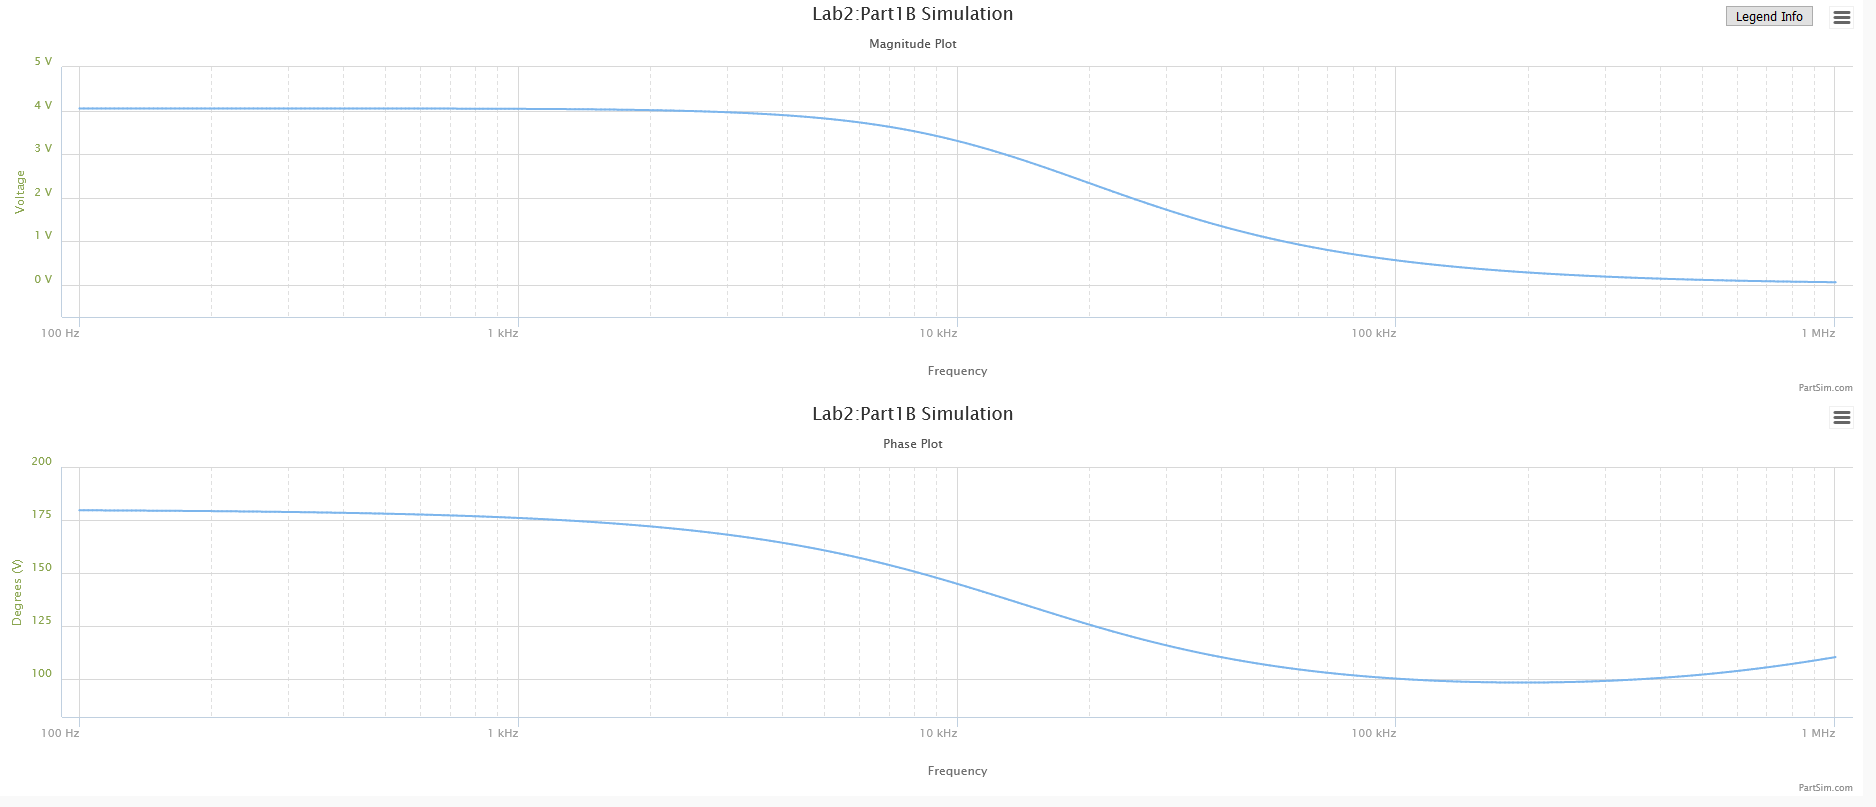
\includegraphics[width=\textwidth]{Step1.7}
        \caption{Bode plots of intrinsic voltage gain $A_{vo}$ (real magnitude and phase in degrees)}
        \label{fig:Step1.7}
    \end{figure}
    \begin{figure}[!ht]
        \centering
        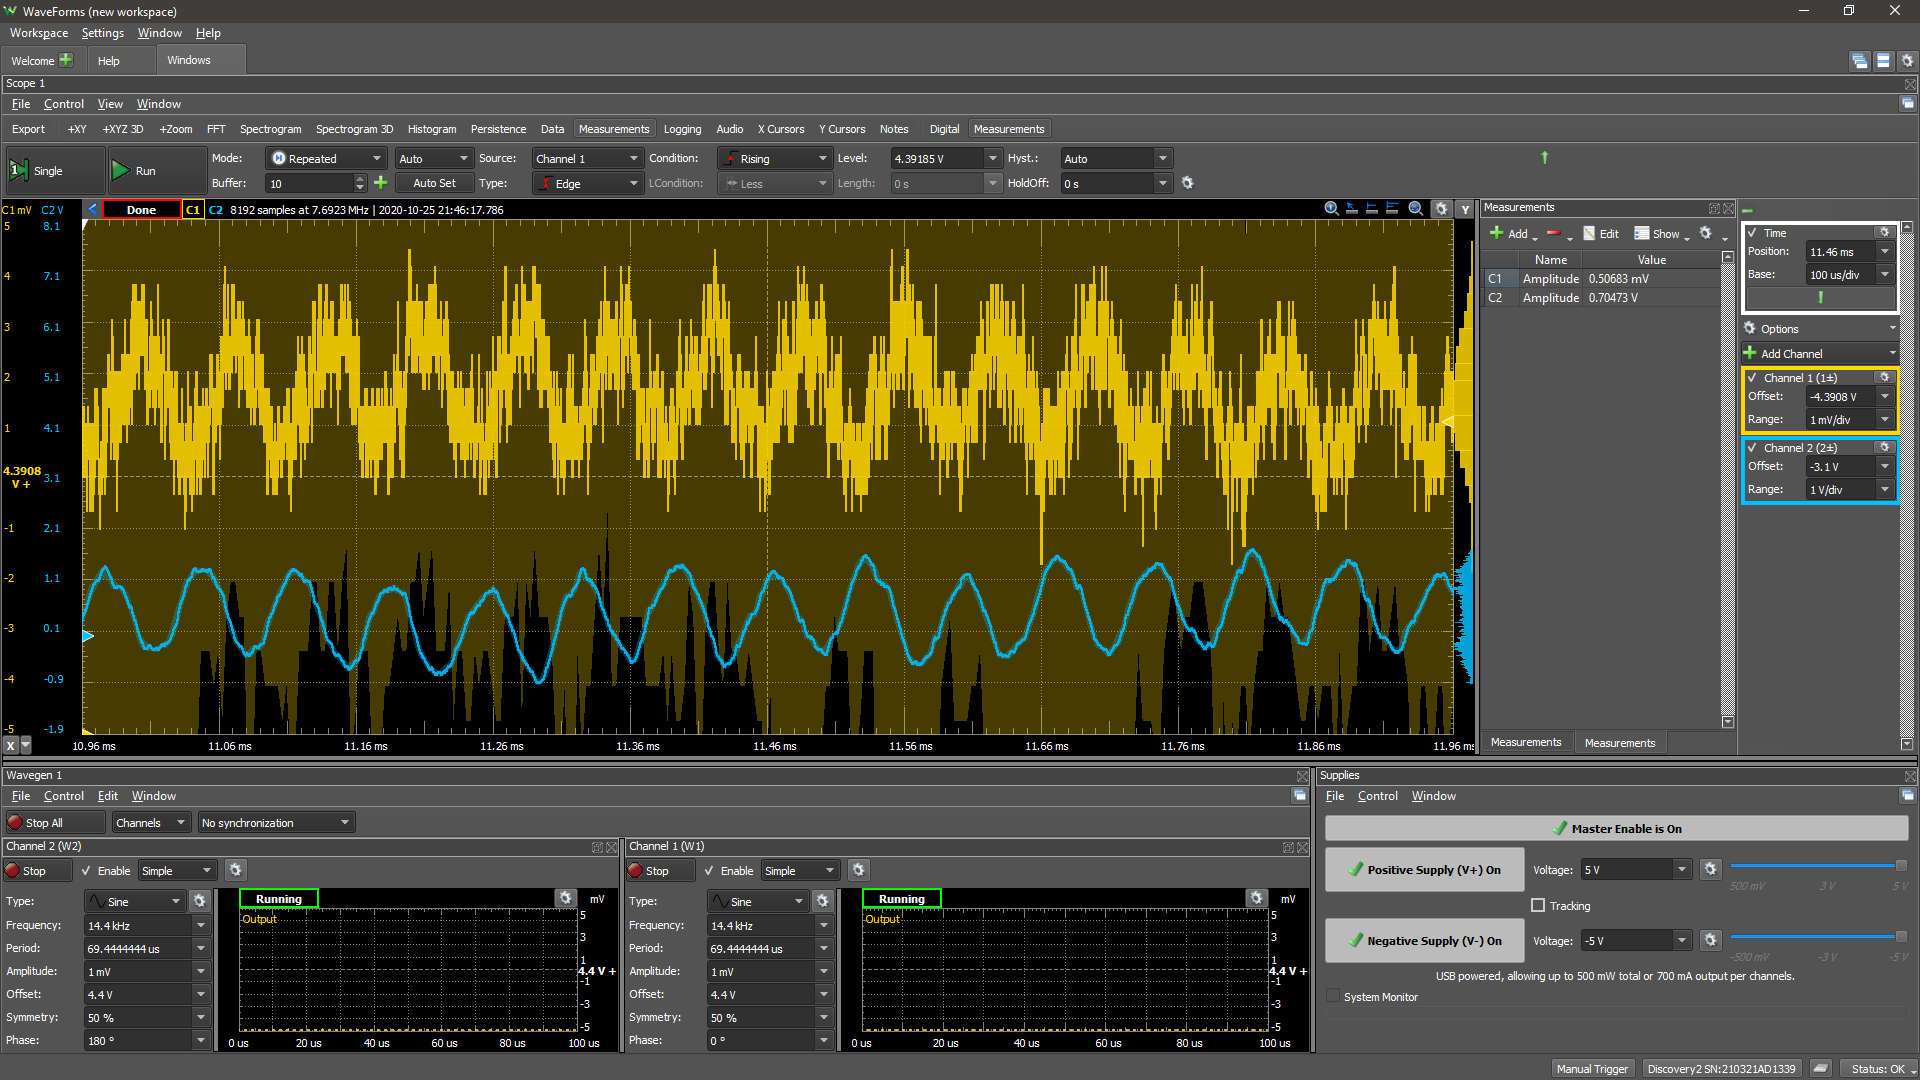
\includegraphics[width=\textwidth]{Q4.3}
        \caption{WaveForms screenshot for Q4.3}
        \label{fig:Q4.3}
    \end{figure}
    \pagebreak
    \section*{Part 2}
    % A) Prelab: ~2.1, ~2.2, ~2.3
    % B) In-lab: 2.4, 2.5, 2.6, 2.7, 2.8, 2.9
    \item [\textbf{Q5.}]
    \begin{enumerate}
        \item The simulated $V_o$ vs $V_{sig}$ characteristics are shown in Figure \ref{fig:Step2.2}. The measured $V_o$ vs $V_{sig}$ characteristics are shown in Figure \ref{fig:Step2.6}. The characteristics align with the expected characteristics of a common-collector amplifier, a near linear 1:1 voltage ratio due to the voltage gain being nearly zero.
        \begin{figure}[!ht]
            \centering
            \begin{subfigure}[b]{0.45\textwidth}
                \centering
                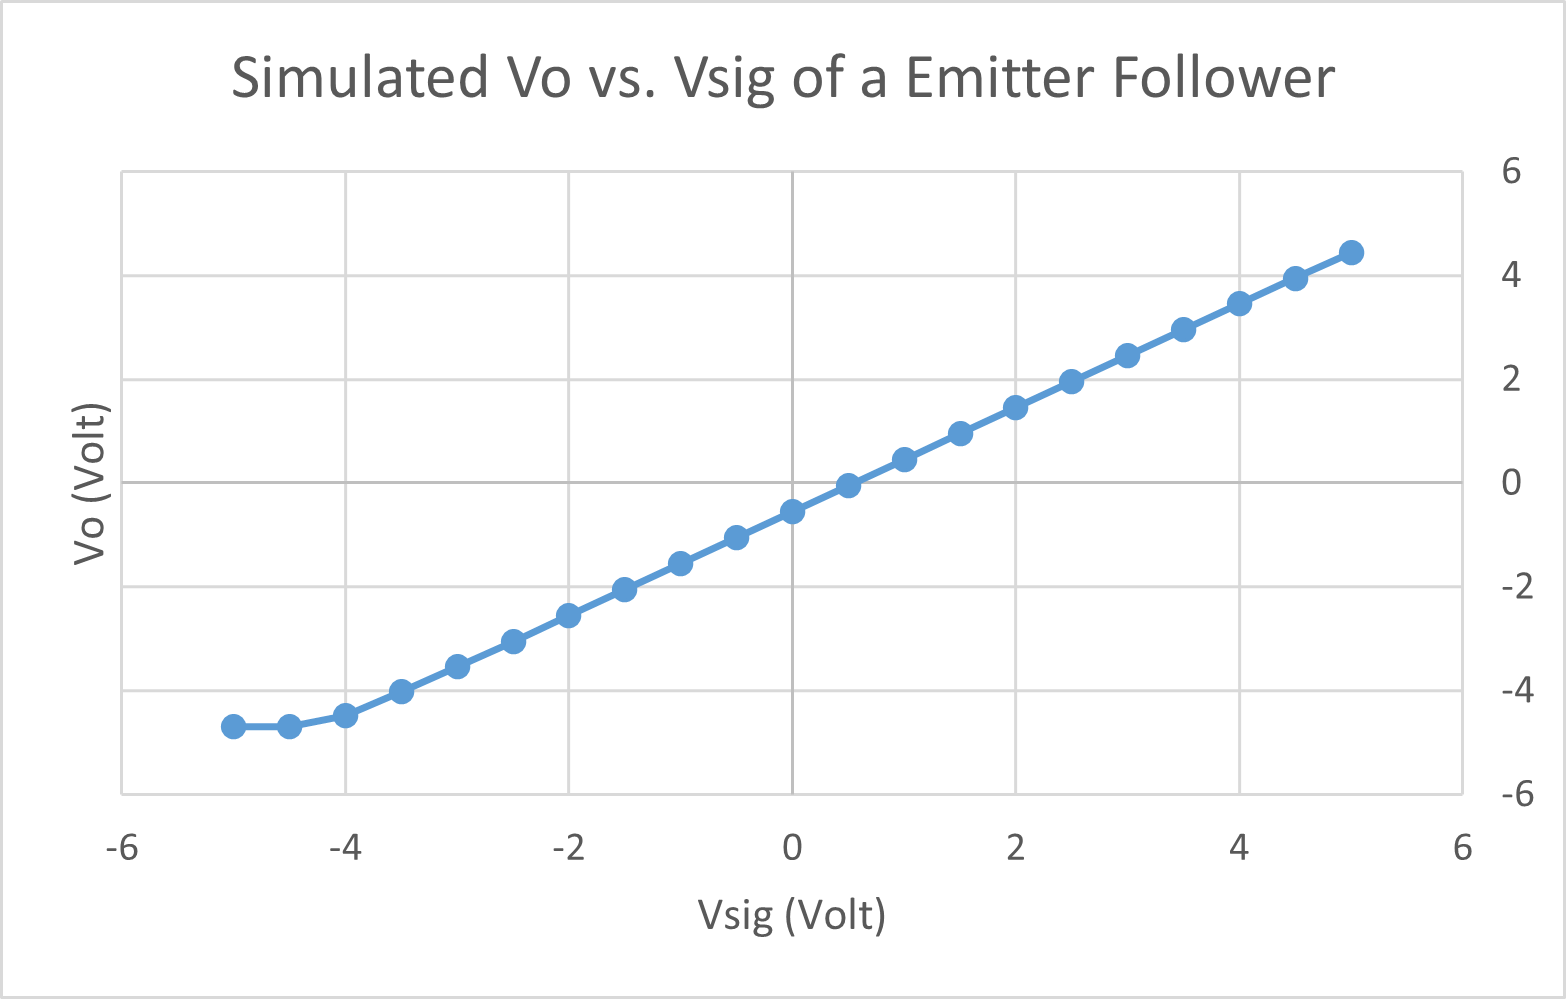
\includegraphics[width=\textwidth]{Step2.2}
                \caption{Step 2.2}
                \label{fig:Step2.2}
            \end{subfigure}
            \begin{subfigure}[b]{0.48\textwidth}
                \centering
                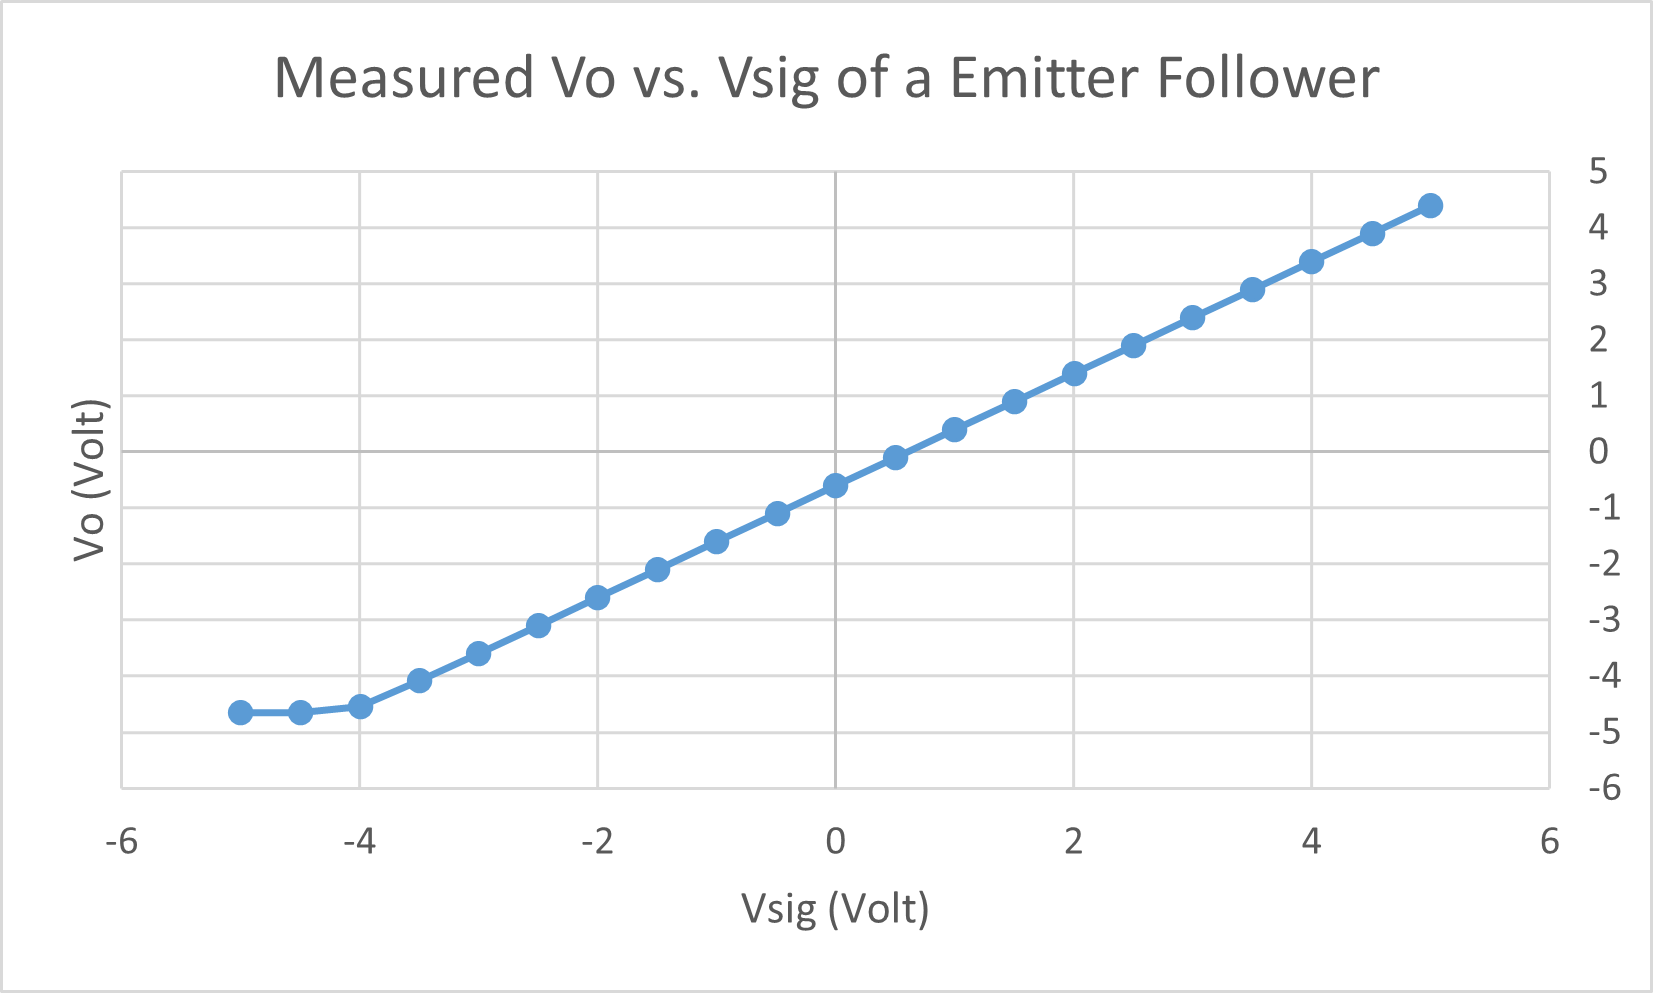
\includegraphics[width=\textwidth]{Step2.6}
                \caption{Step 2.6}
                \label{fig:Step2.6}
            \end{subfigure}
            \caption{$V_o$ vs $V_{sig}$ characteristics}
        \end{figure}
        \item The DC input range for $V_{sig}$ was found to be $V_{sig} > -4$ V and the voltage range for $V_o$ was found to be around $V_o > 4.5$ V.
        \item The value of $V_{sig}$ that results in $V_o \approx 0$ V was found to be approximately 0.6 V.
    \end{enumerate}
    \item [\textbf{Q6.}]
    Based on the simulation data obtained in Step 2.3, the magnitude and phase of the simulated intrinsic voltage gain $A_{vo}$ at low frequency are $-60$ dB and 0\degree. Based on the measurement data obtained in Step 2.8, the magnitude and phase of the measured intrinsic voltage gain $A_{vo}$ at low frequency was determined to be 0 dB and 0\degree. The simulated bode plots for the intrinsic voltage gain $A_{vo}$ (real magnitude and phase in degrees) is shown in Figure \ref{fig:Step2.3}.
    \begin{figure}[!ht]
        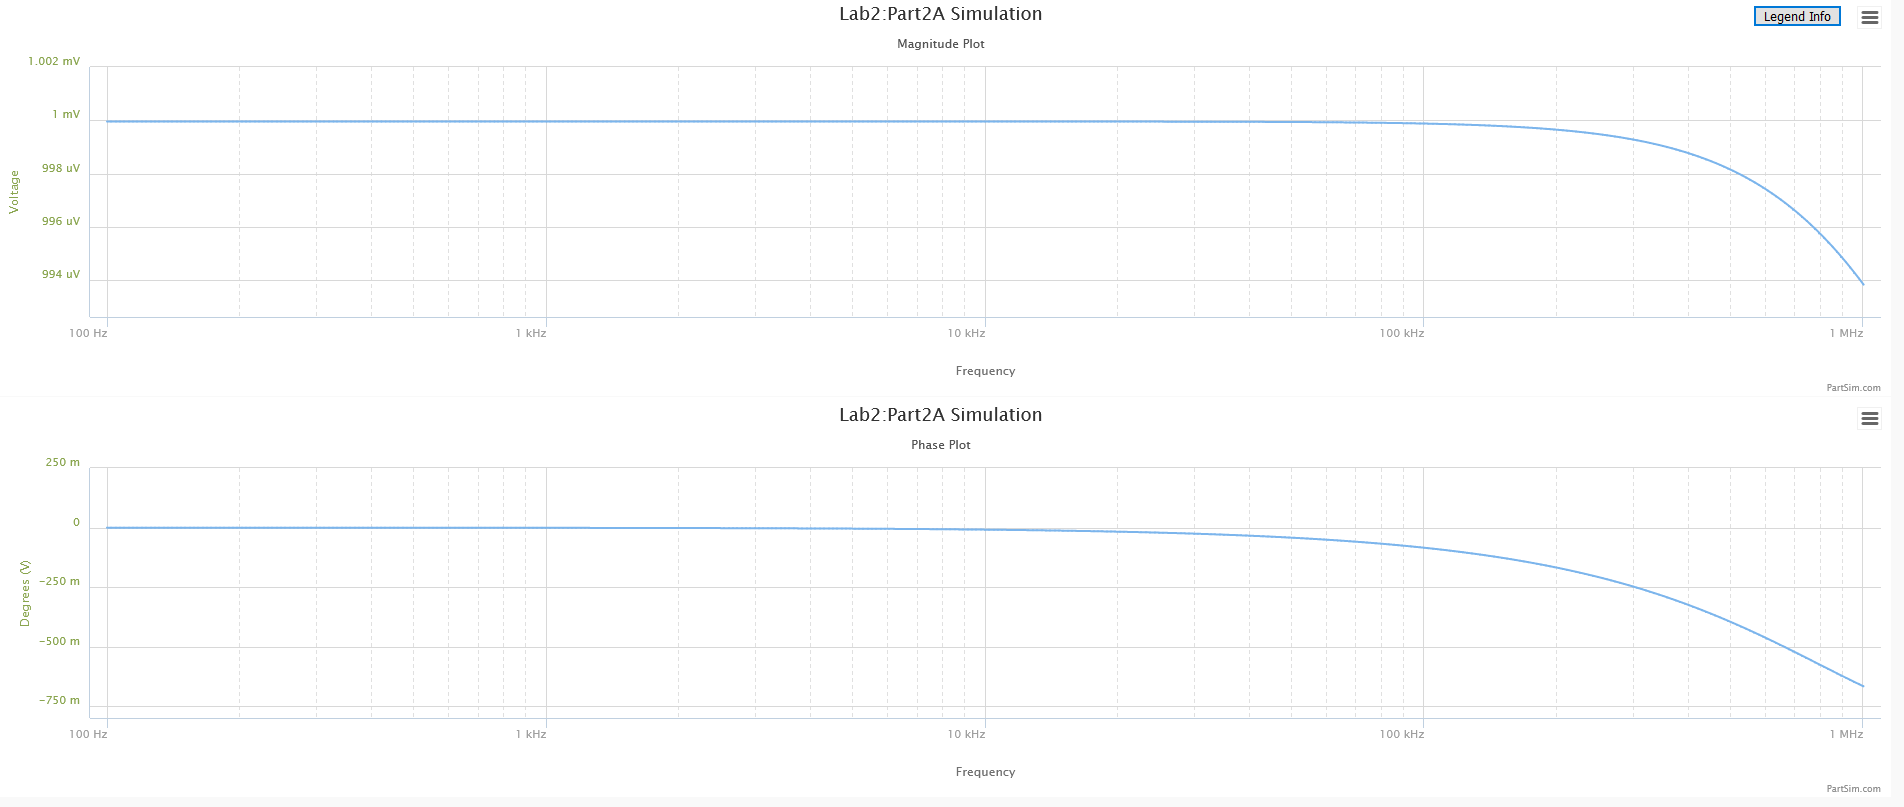
\includegraphics[width=\textwidth]{Step2.3}
        \caption{Bode plots for the intrinsic voltage gain $A_{vo}$ (real magnitude and phase in degrees)}
        \label{fig:Step2.3}
    \end{figure}
    \pagebreak
    \section*{Part 3}
    % A) Prelab: ~3.1, ~3.2, ~3.3
    % B) Prelab: ~3.4, ~3.5, ~3.6
    \item [\textbf{Q7.}]
    \begin{enumerate}
        \item $V_o = 4.25$ V, $V_e = -0.525$V, $I_{C2} = 90.91\mu$A. A plot of the simulated data is shown in Figure \ref{fig:Step3.2}.
        \begin{figure}[!ht]
            \centering
            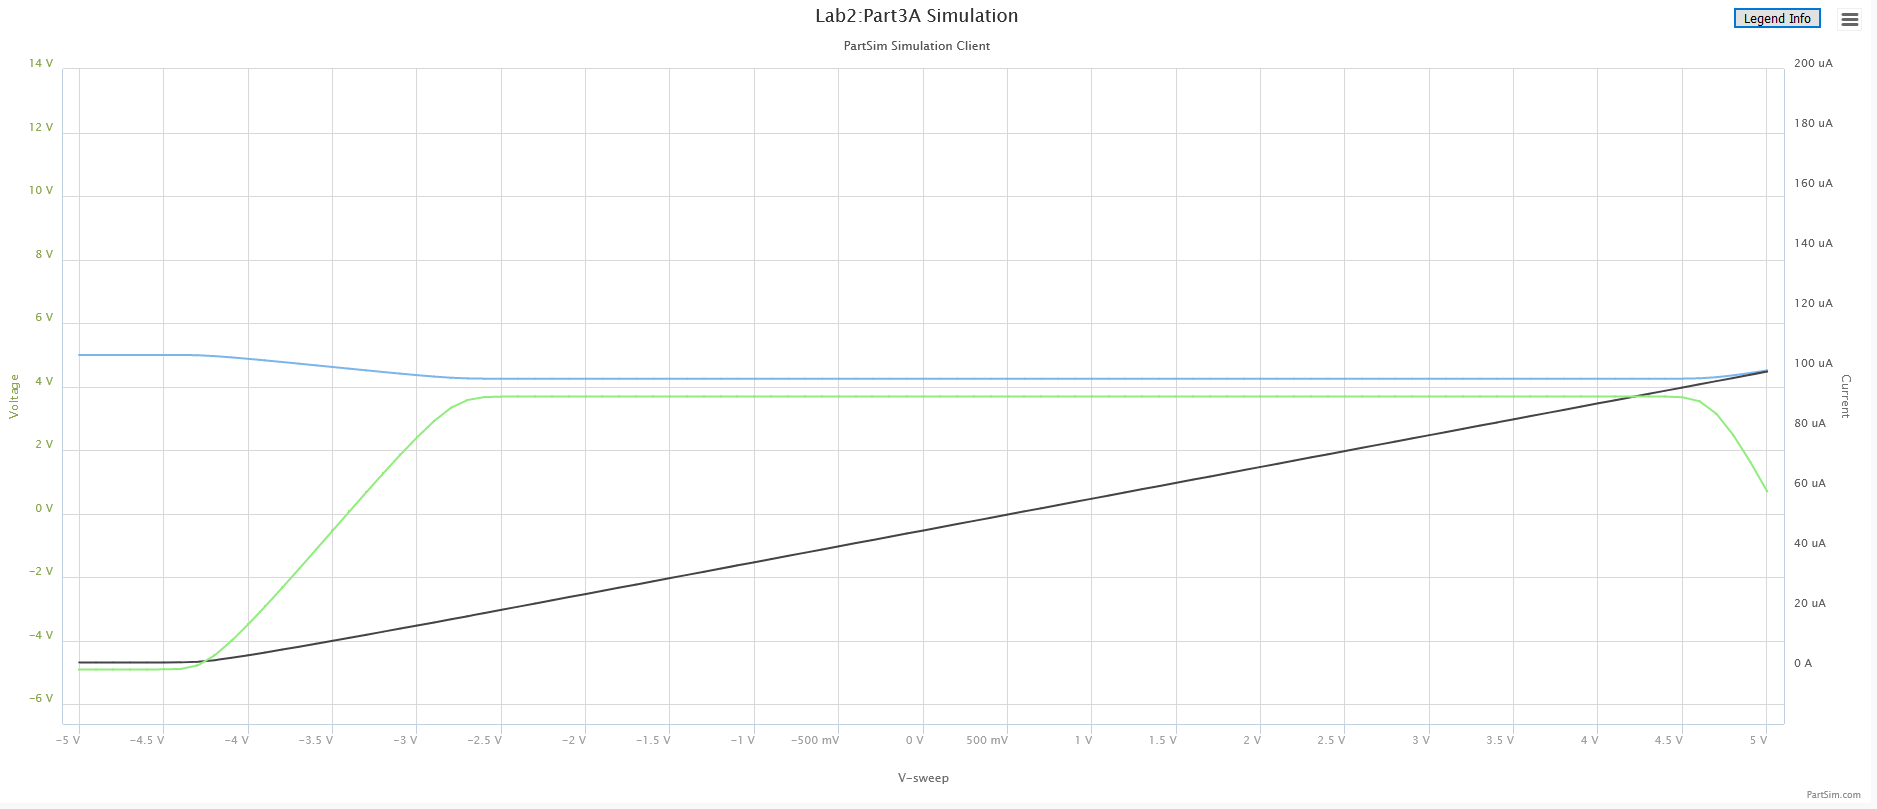
\includegraphics[width=\textwidth]{Step3.2}
            \caption{Step 3.2}
            \label{fig:Step3.2}
        \end{figure}
        \item The input common-mode range is $-2.7$ V $< V_{CM} < 4.7$ V
        \item The upper and lower bounds of the input common-mode range are determined by the regions where the BJT's collector current and output voltage are constant.
        \setcounter{enumi}{4} \item The input common-mode range determined using the measured data was $-2.7$ V $< V_{CM} < 4.7$ V, the same as the range determined in simulation. The plots of the measured data are shown in Figure \ref{fig:Q7}.
        \begin{figure}[!ht]
            \centering
            \begin{subfigure}[b]{0.46\textwidth}
                \centering
                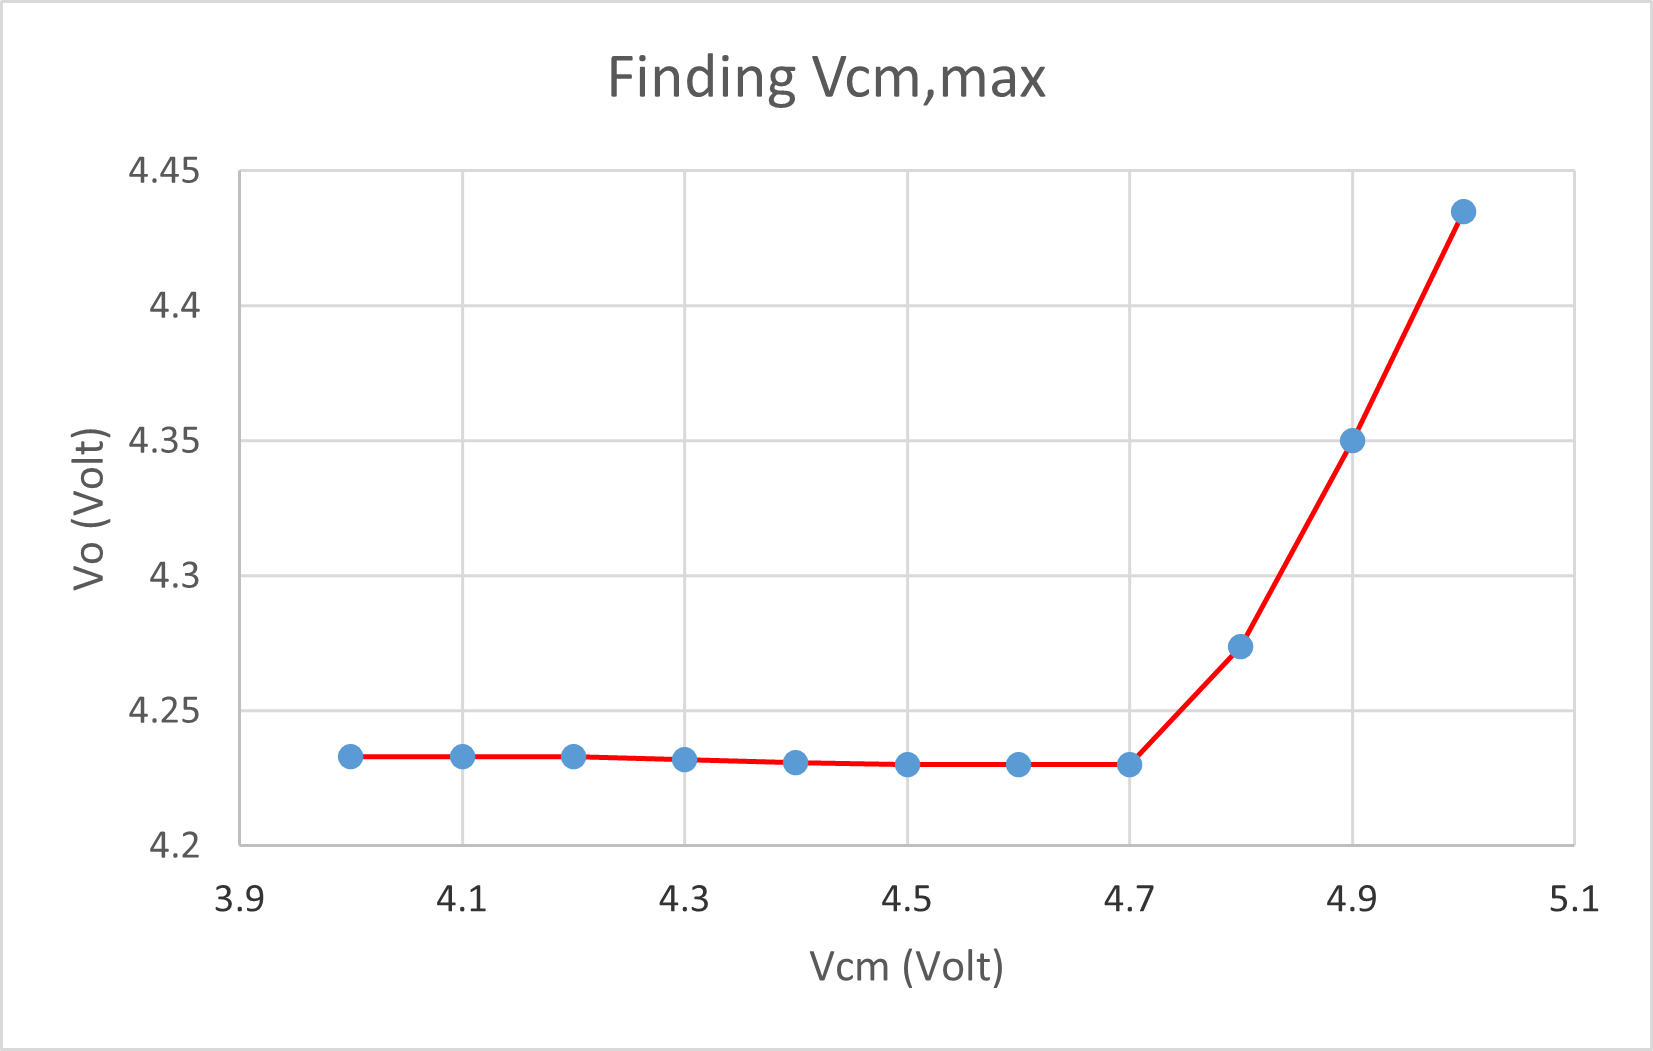
\includegraphics[width=\textwidth]{Step3.10}
                \caption{Step 3.10}
                \label{fig:Step3.10}
            \end{subfigure}
            \begin{subfigure}[b]{0.49\textwidth}
                \centering
                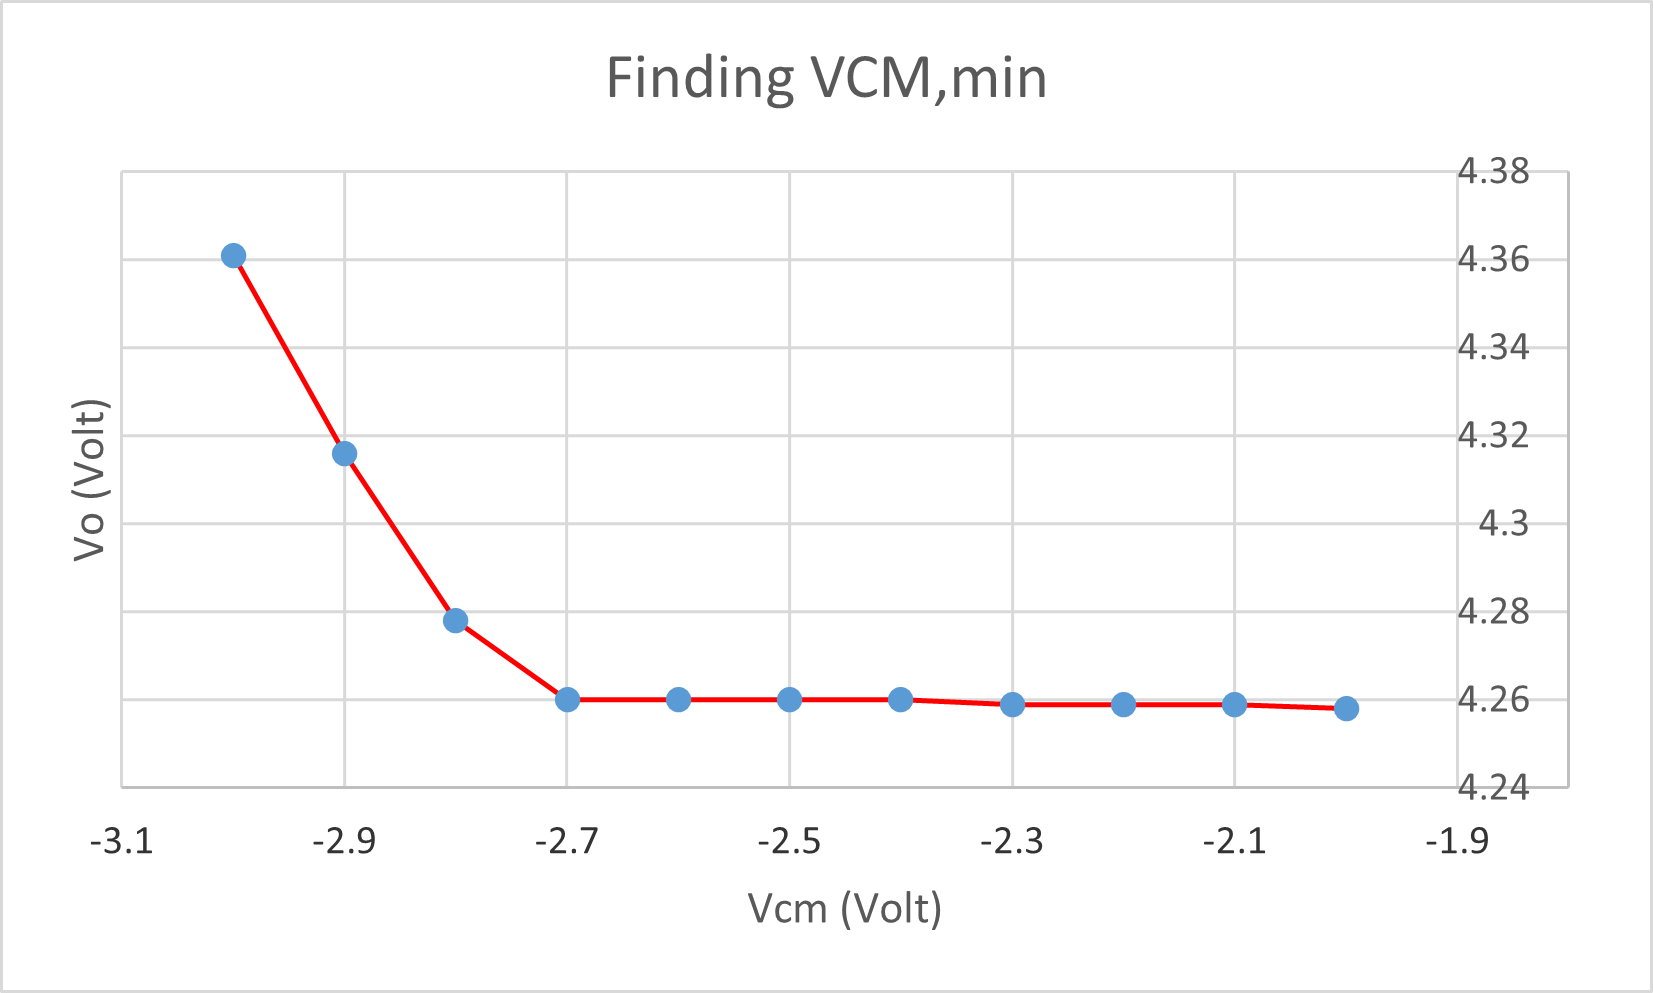
\includegraphics[width=\textwidth]{Step3.11}
                \caption{Step 3.11}
                \label{fig:Step3.11}
            \end{subfigure}
            \caption{Input common-mode range}
            \label{fig:Q7}
        \end{figure}
    \end{enumerate}
    \item [\textbf{Q8.}]
    The low-frequency voltage gain $A_{cm}$ in dB for the common-mode signal was determined to be approximately -147 dB. The bode plots of voltage gain $A_{cm}$ with real magnitude and phase in degrees are shown in Figure \ref{fig:Step3.3}.
    \begin{figure}[!ht]
        \centering
        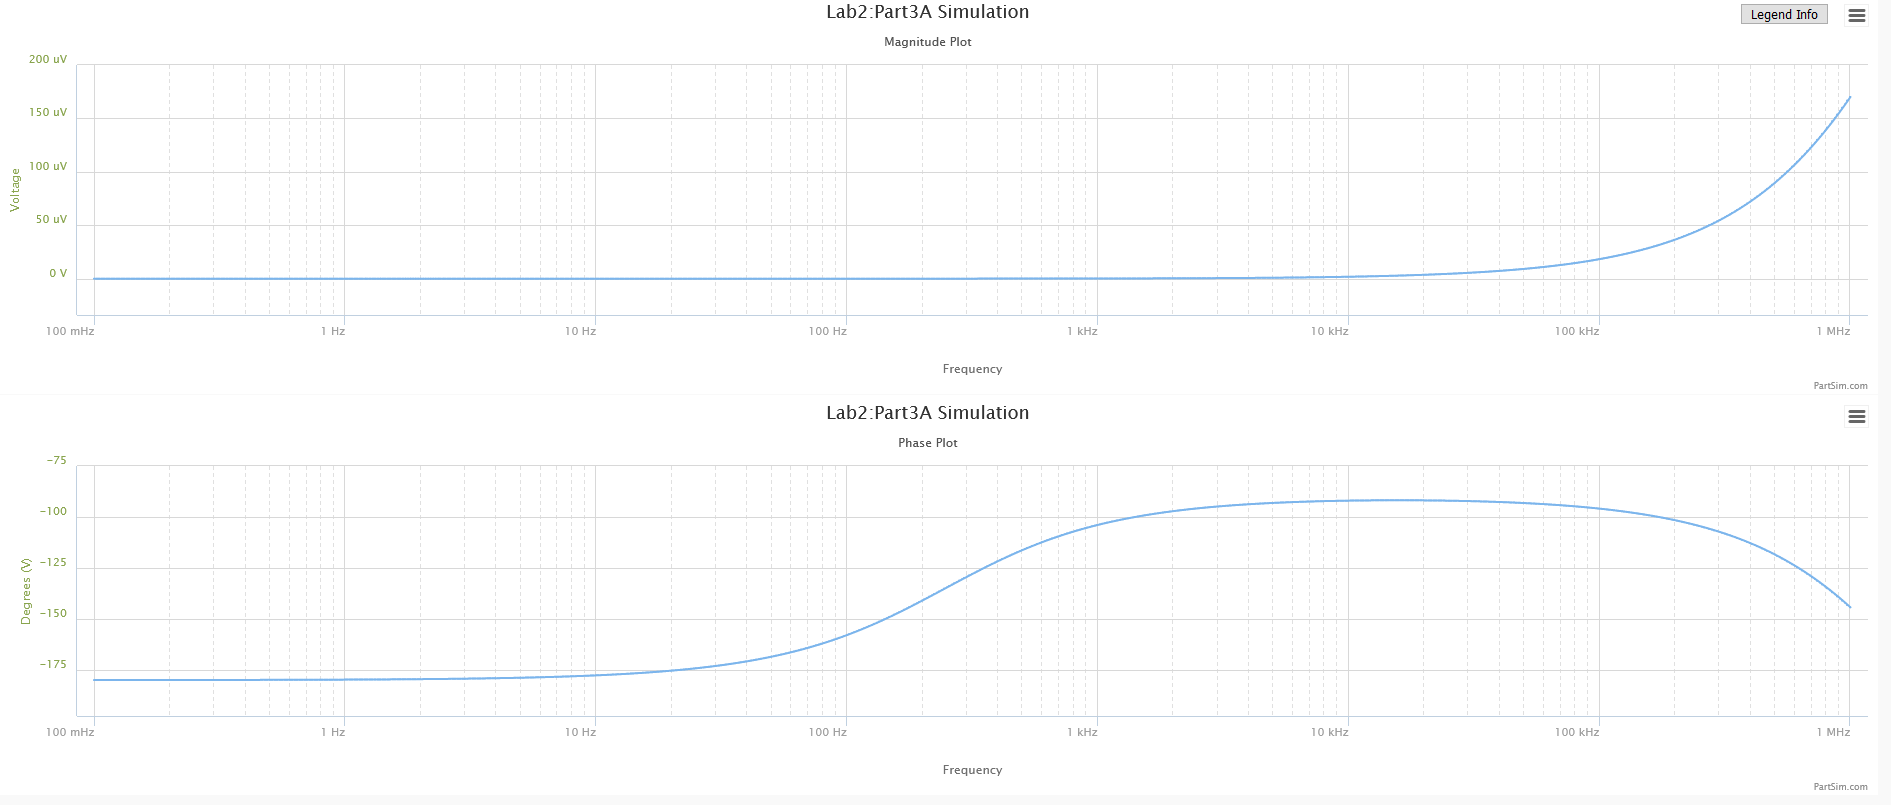
\includegraphics[width=\textwidth]{Step3.3}
        \caption{Bode plots for the voltage gain $A_{cm}$ (real magnitude and phase in degrees)}
        \label{fig:Step3.3}
    \end{figure}
    \item [\textbf{Q9.}]
    The simulation data for Step 3.5 is shown in Figure \ref{fig:Step3.5}.
    \begin{enumerate}
        \item The input differential-mode range was determined to be approximately $-0.06$ V $< V_{id} < 0.06$ V.
        \item The upper and lower bounds are determined by finding the value of $V_{id}$ that causes most of the current to flow through a single BJT (approximately 0.12 V), and dividing this value by 2.  
    \end{enumerate}
    \begin{figure}[!ht]
        \centering
        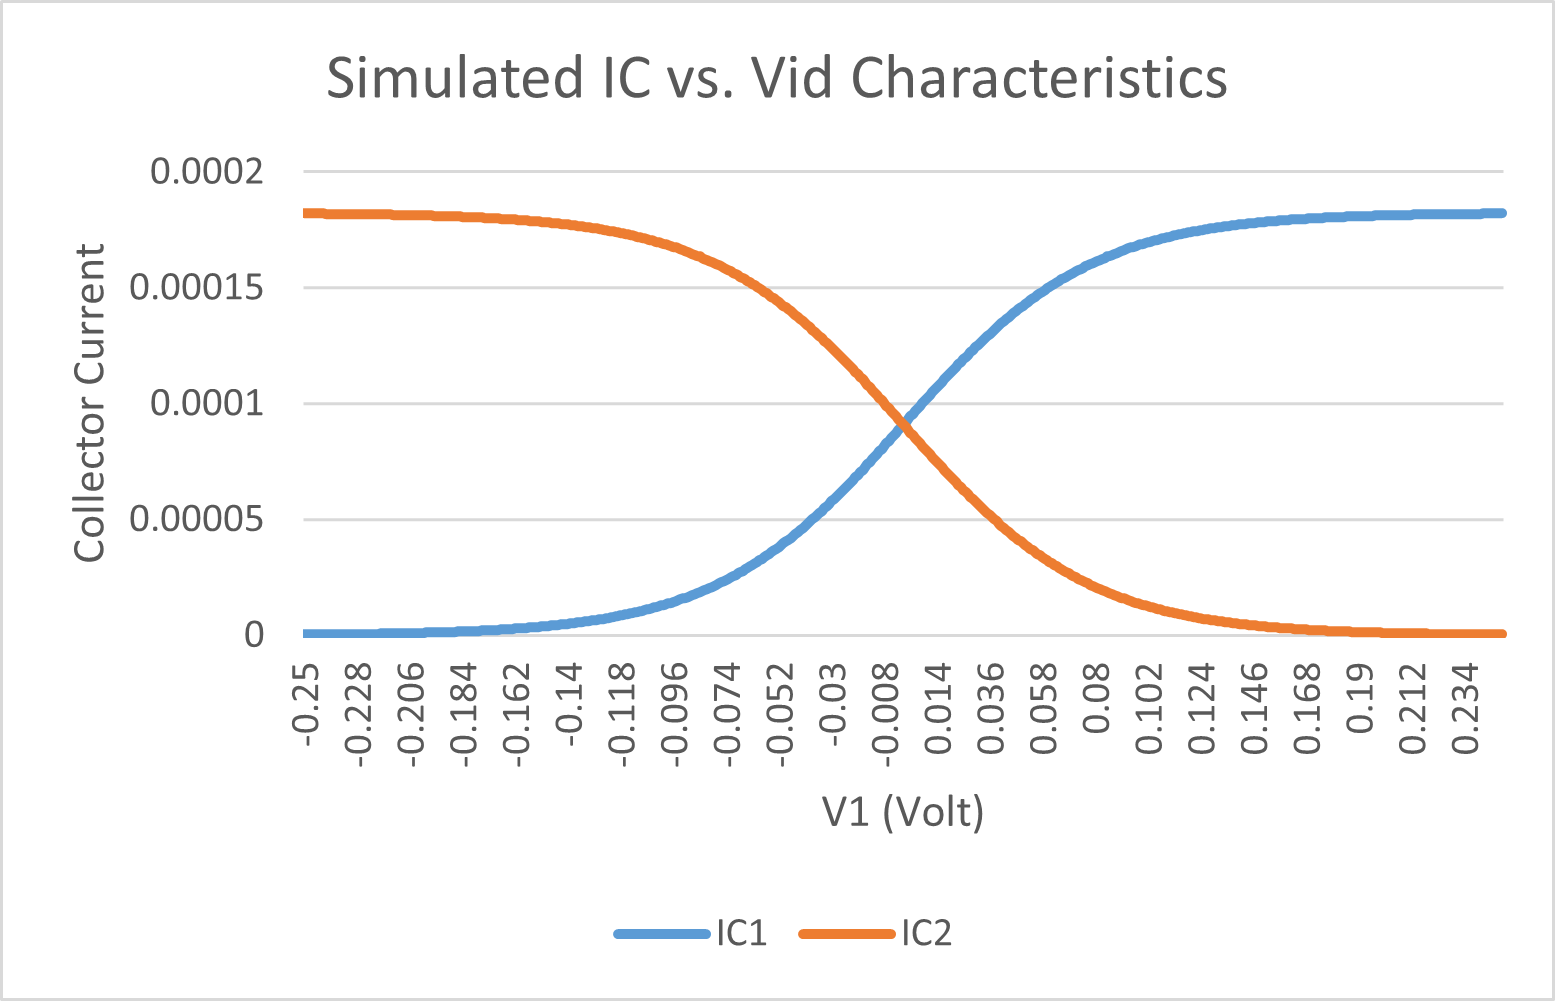
\includegraphics[width=0.68\textwidth]{Step3.5}
        \caption{Step 3.5}
        \label{fig:Step3.5}
    \end{figure}
    \item [\textbf{Q10.}]
    \begin{enumerate}
        \item The voltage gain $A_d$ in dB is -34.352 dB. The bode plots of voltage gain $A_{d}$ with real magnitude and phase in degrees are shown in Figure \ref{fig:Step3.6}.
        \begin{figure}[!ht]
            \centering
            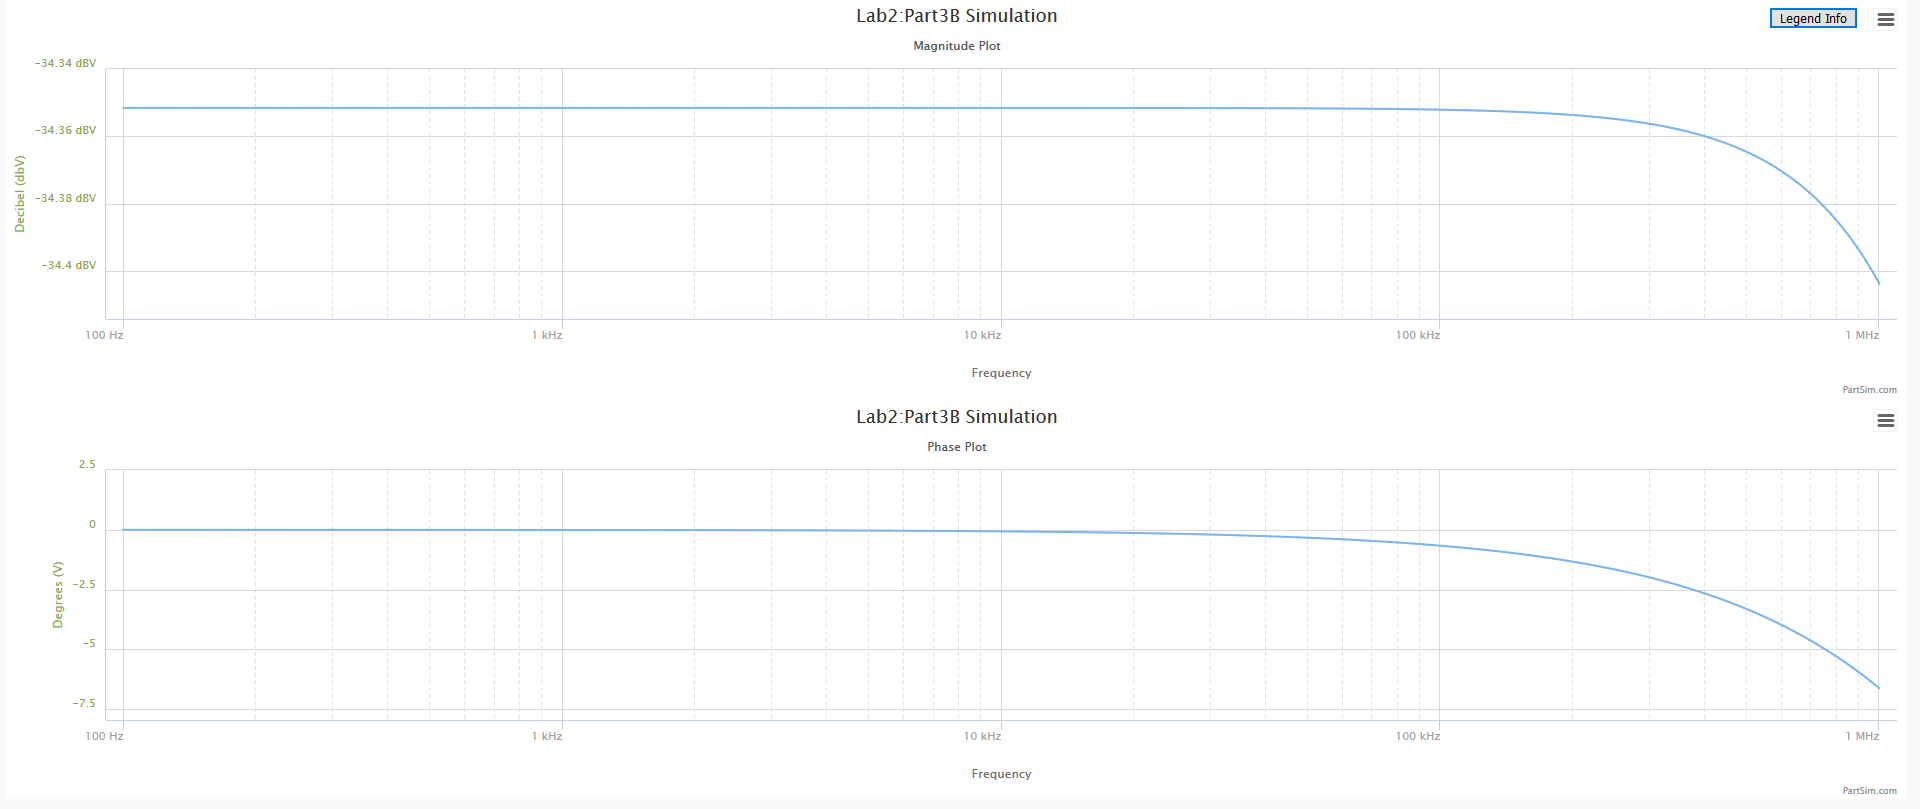
\includegraphics[width=\textwidth]{Step3.6}
            \caption{Bode plots for the voltage gain $A_{d}$ (real magnitude and phase in degrees)}
            \label{fig:Step3.6}
        \end{figure}
        \item The DC analysis was extended to stop at a frequency of 10 MHz, and the upper 3-dB frequency was found to be approximately 8.4 MHz.
        \item The upper 3-dB frequency of this differential amplifier is extremely large (3 magnitudes greater) in comparison to the upper 3-dB frequency of the CE amplifier obtained in Q4 (8.4 MHz vs 14 KHz).
        \item The measured low-frequency differential voltage gain $A_d$ was determined in Step 3.14 to be 20.5 dB.
    \end{enumerate}
    \item [\textbf{Q11.}]
    The common-mode rejection ratio (CMRR), $\frac{|A_d|}{|A_{CM}|}$, was calculated to be approximately 112.5 dB. 
\end{itemize}
\pagebreak
\section*{Appendix}
\begin{figure}[!ht]
    \centering
    \begin{subfigure}[b]{0.33\textwidth}
        \centering
        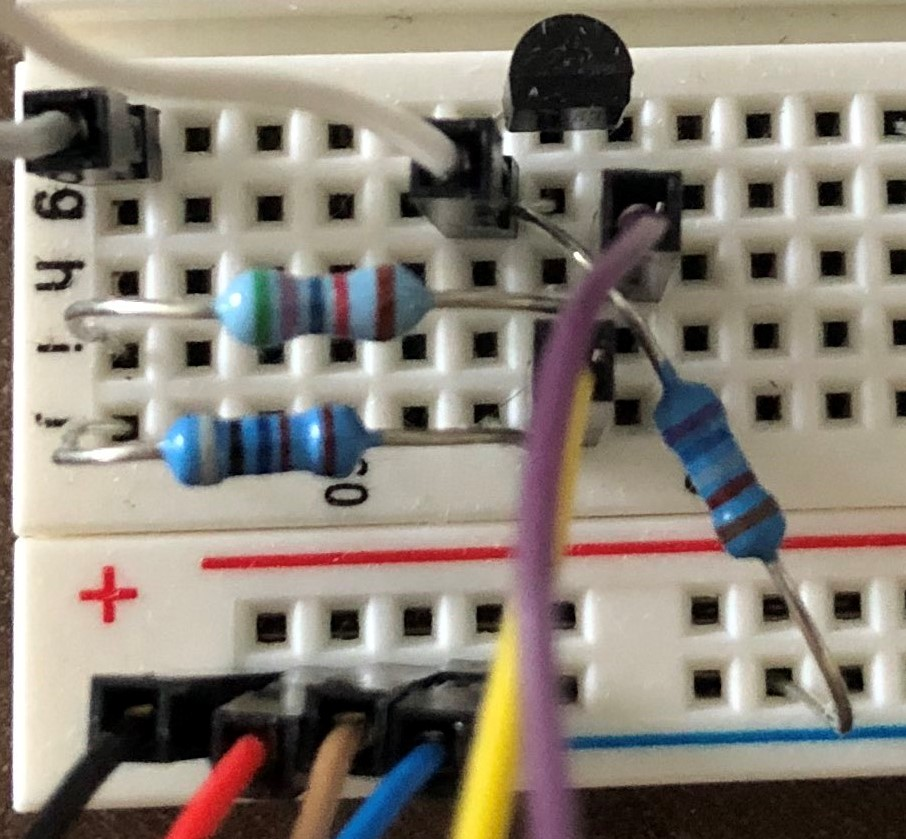
\includegraphics[width=\textwidth]{Part1A}
        \caption{Part 1: C Circuit}
    \end{subfigure}
    \begin{subfigure}[b]{0.45\textwidth}
        \centering
        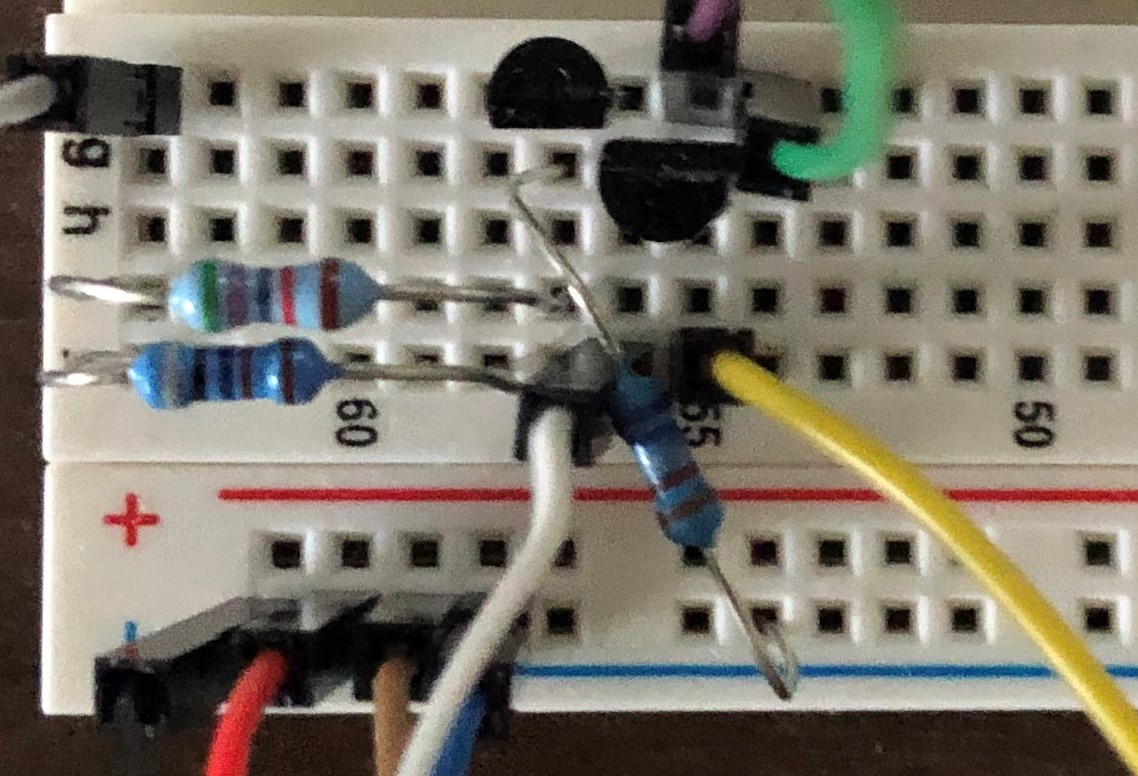
\includegraphics[width=\textwidth]{Part1B}
        \caption{Part 1: D Circuit}
    \end{subfigure}
    \caption{Circuits for Part 1}
\end{figure}
\begin{figure}[!ht]
    \centering
    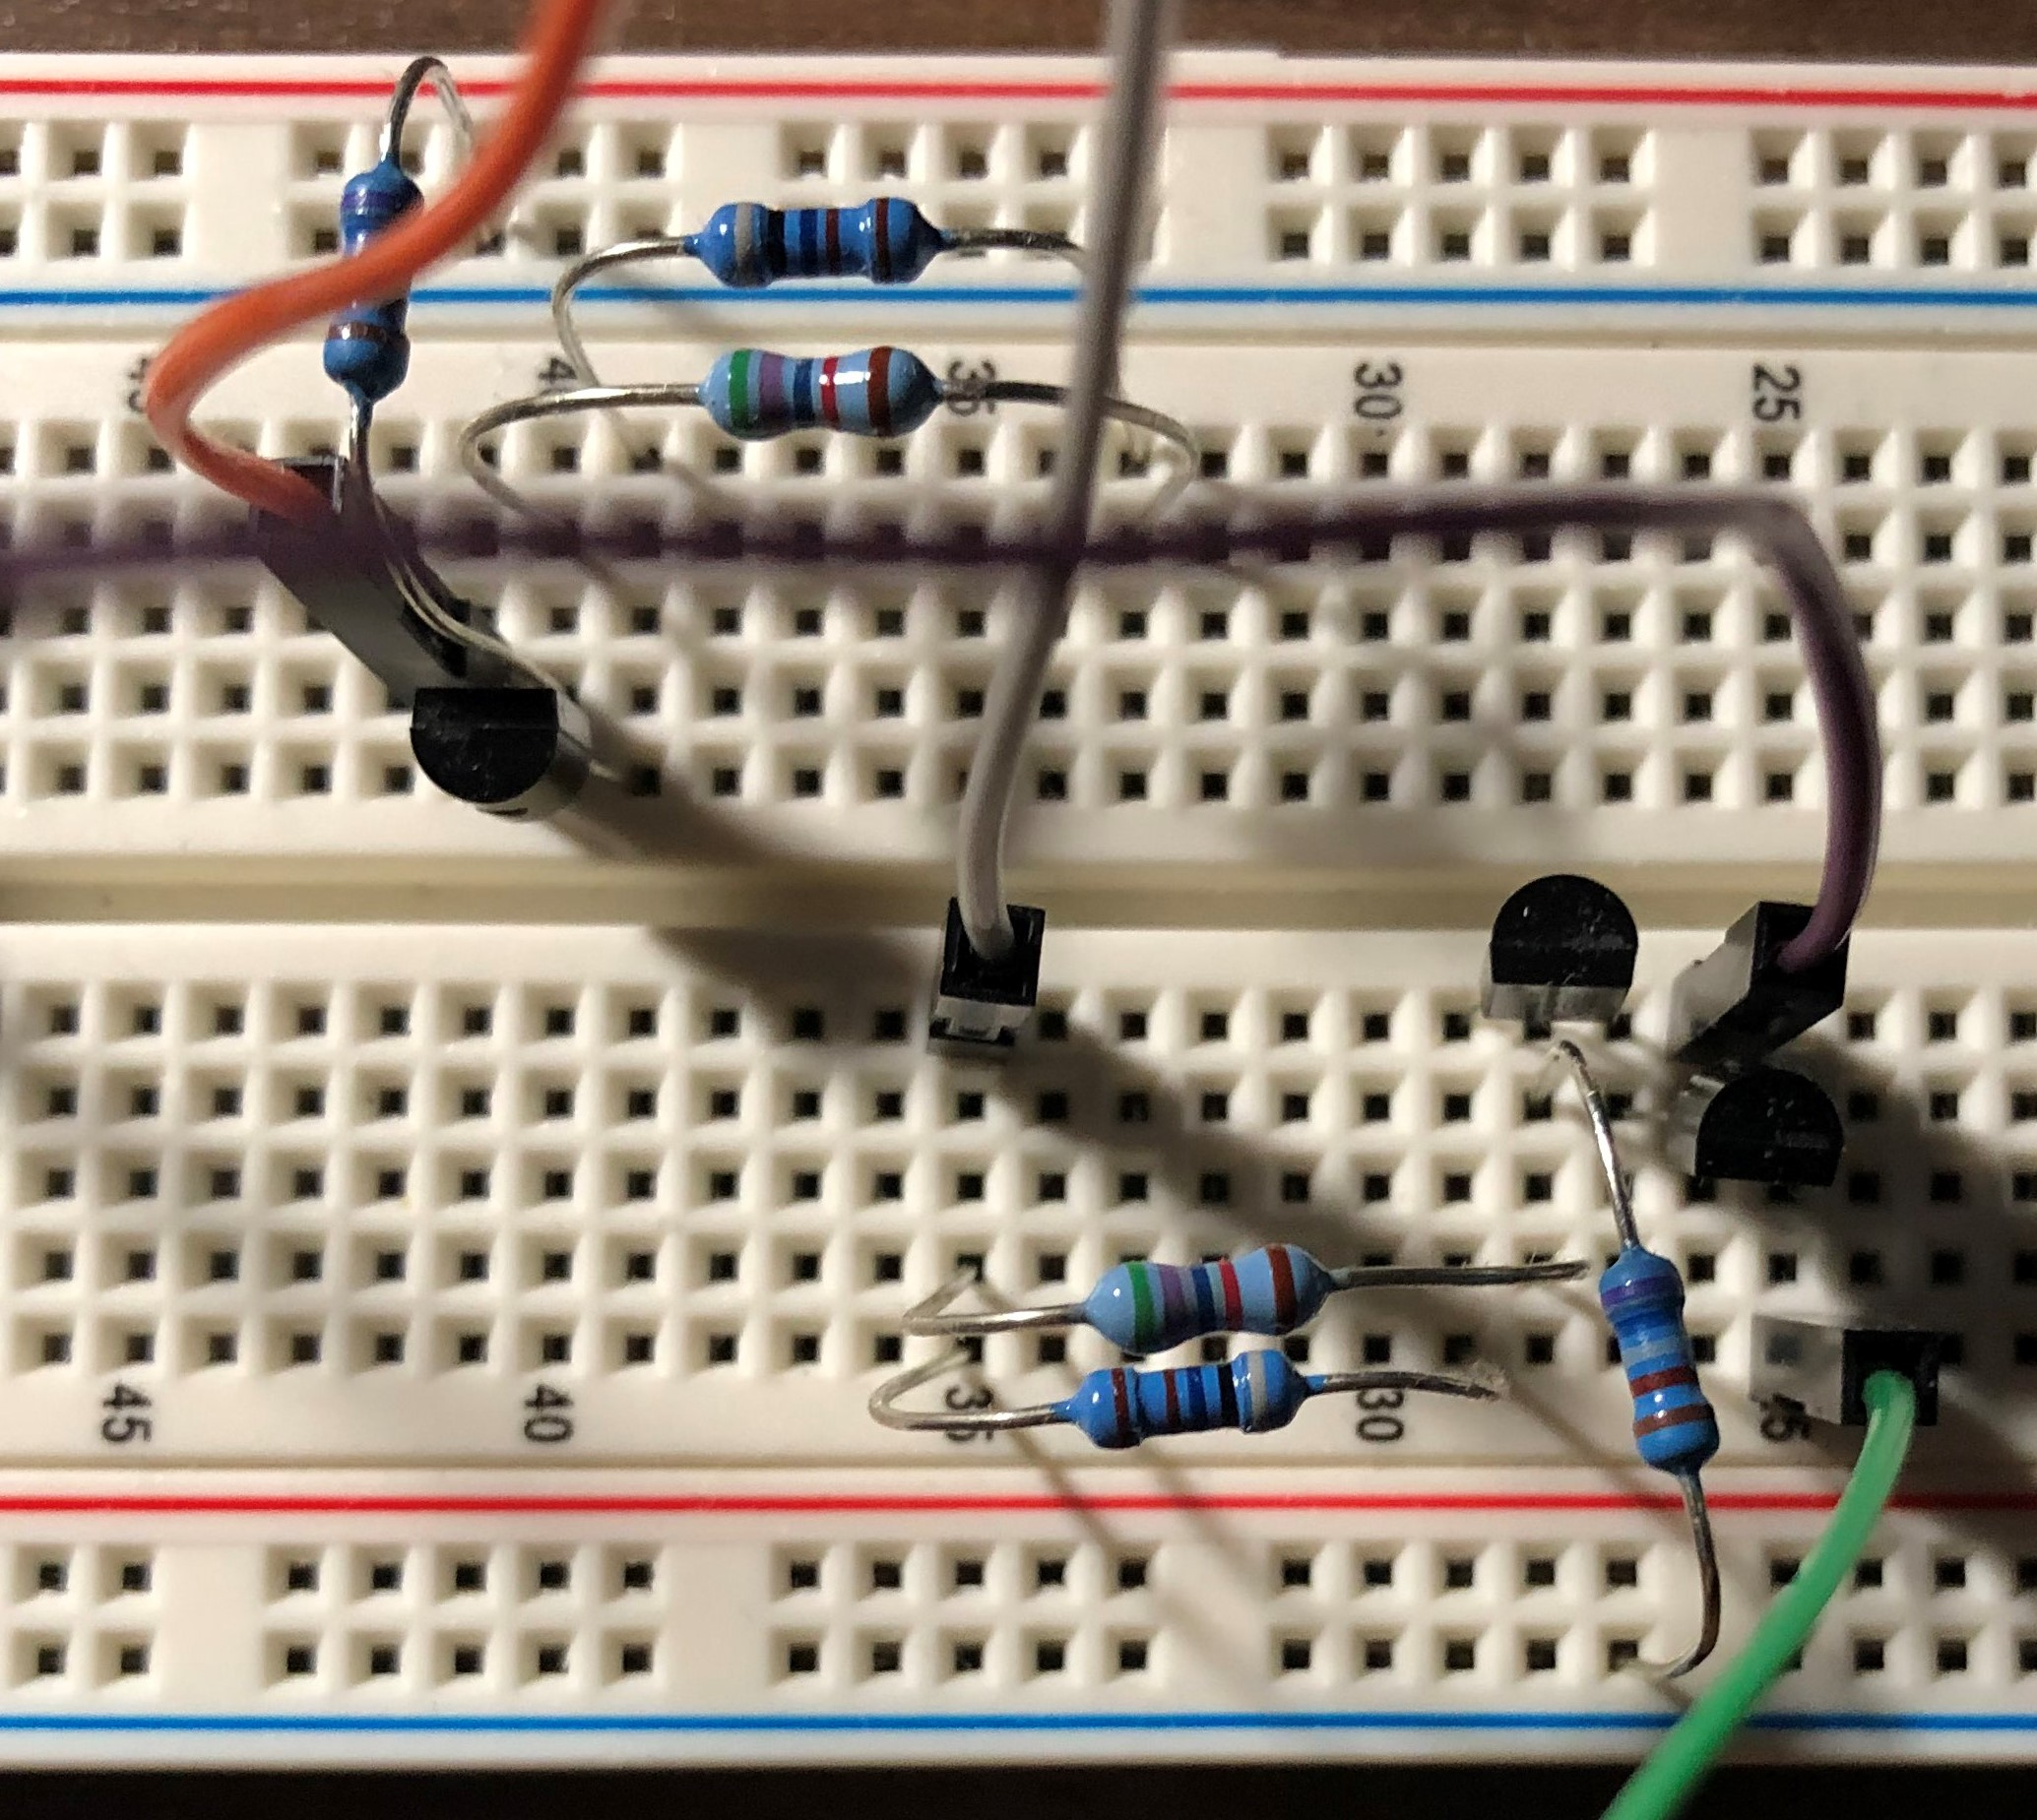
\includegraphics[width=0.4\textwidth]{Part2}
    \caption{Part 2: B Circuit}
\end{figure}
\begin{figure}[!ht]
    \centering
    \begin{subfigure}[b]{0.47\textwidth}
        \centering
        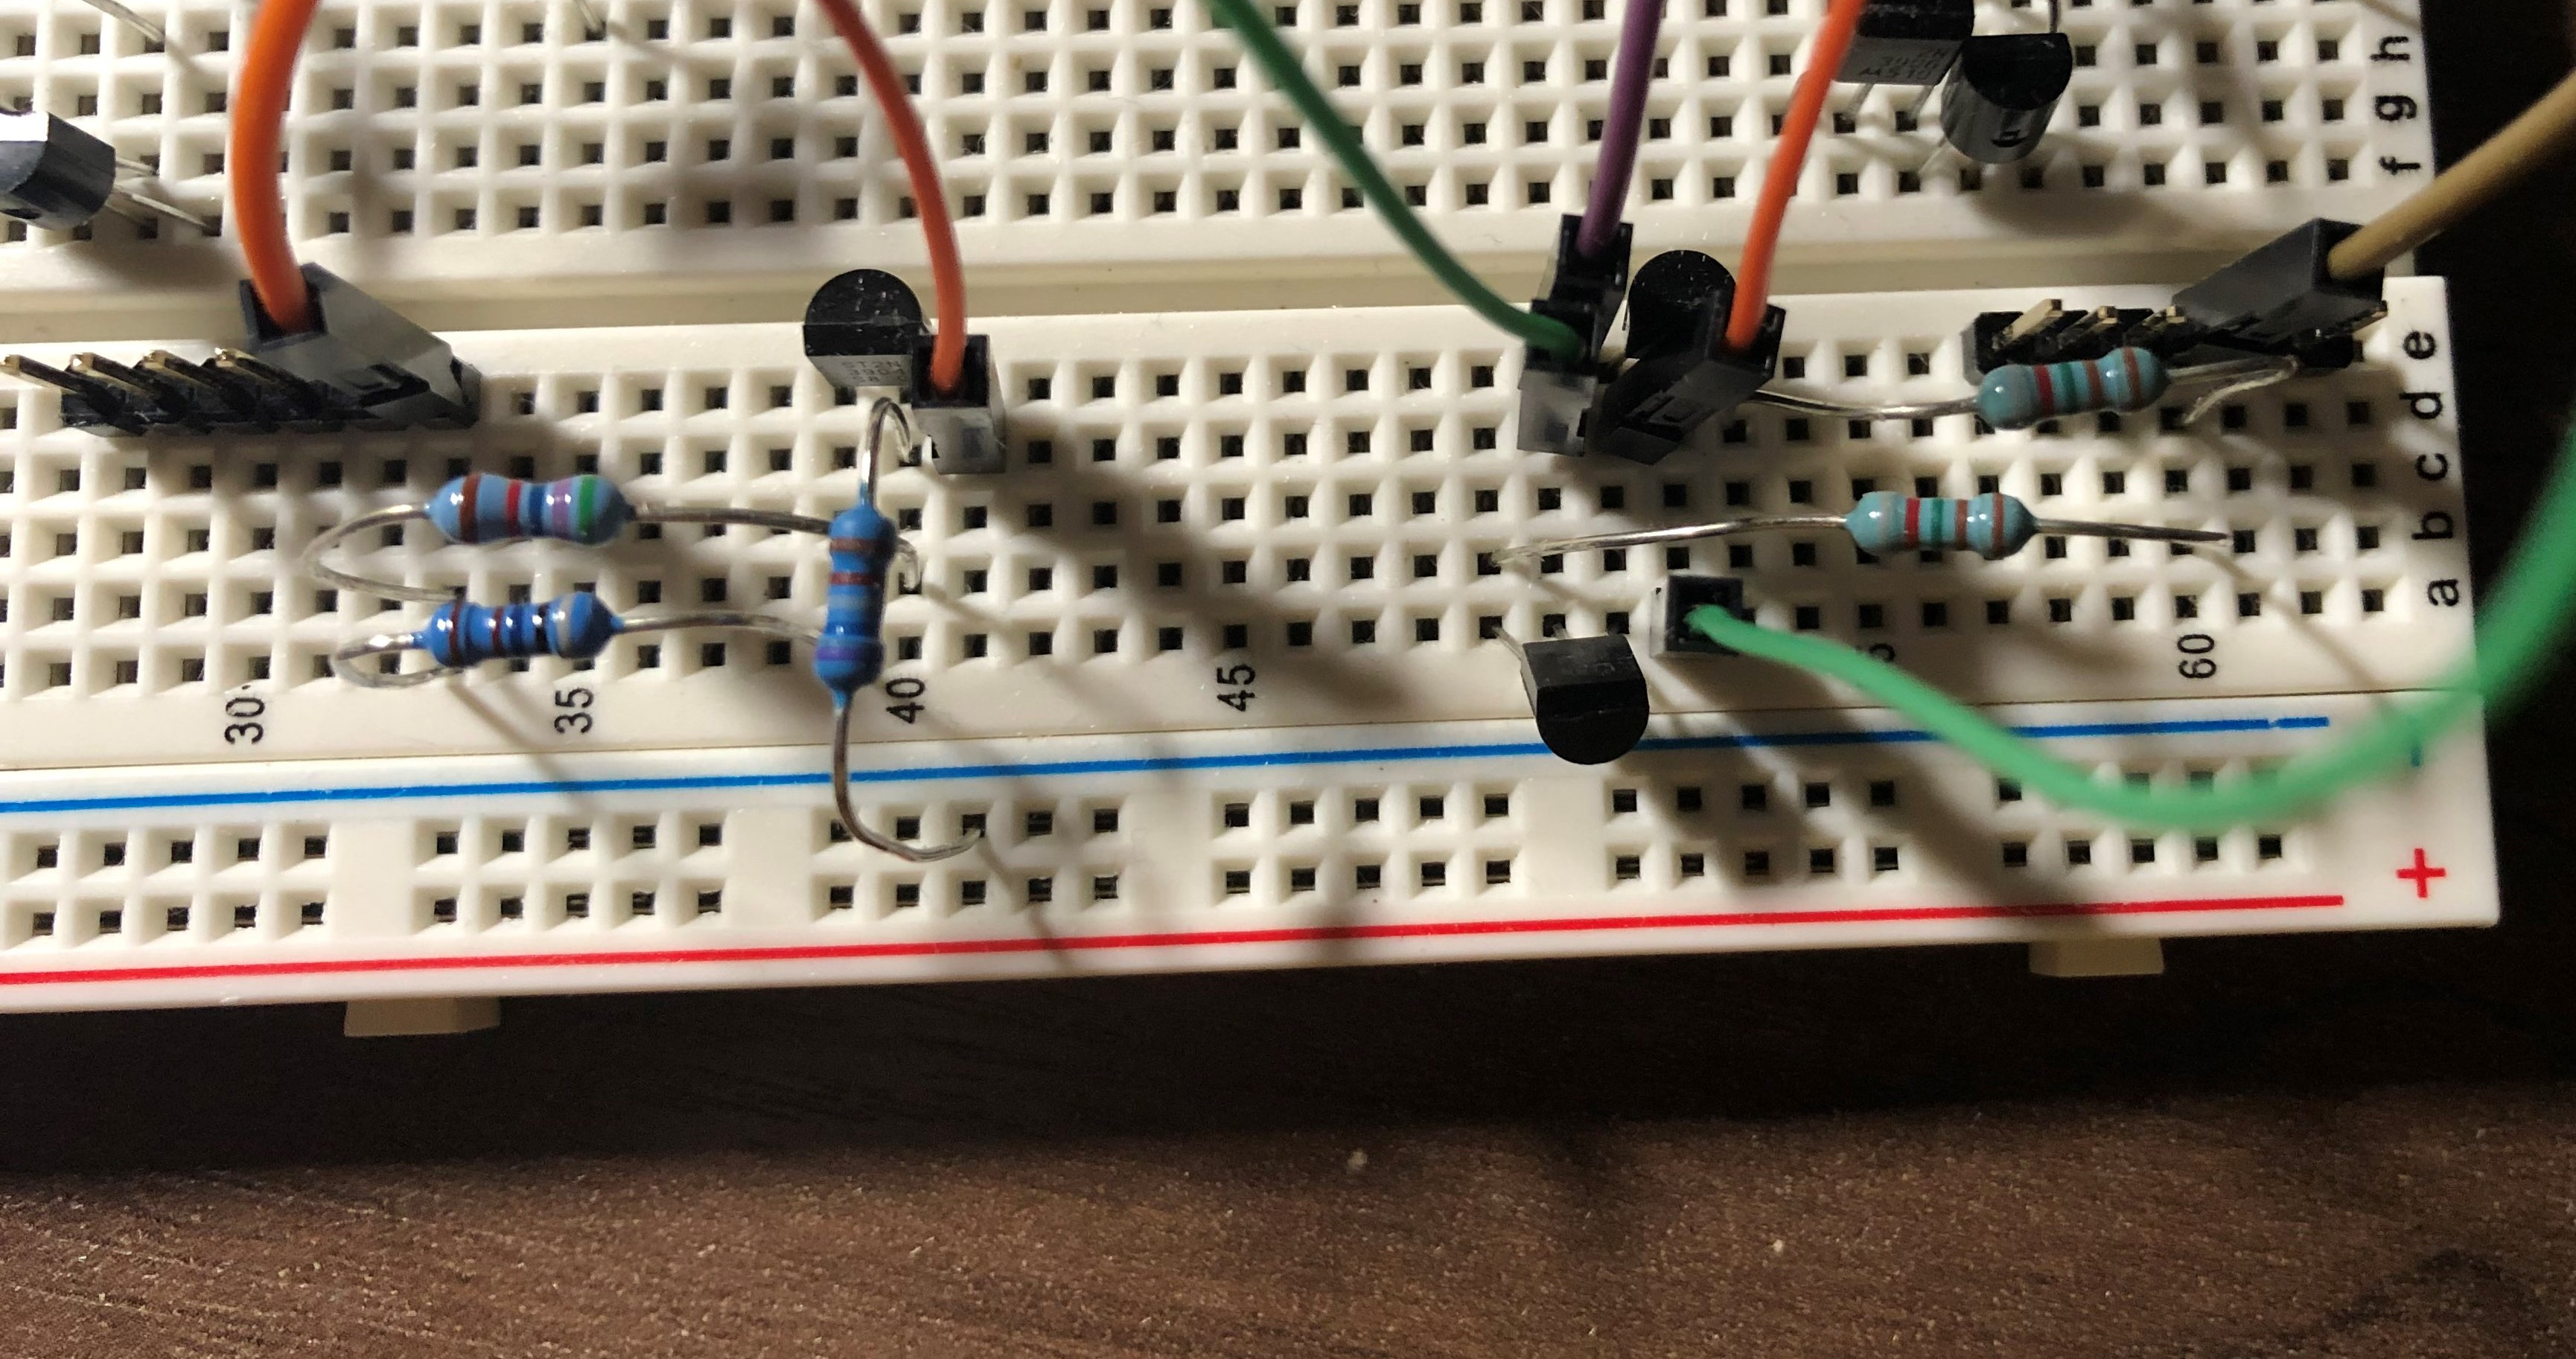
\includegraphics[width=\textwidth]{Part3A}
        \caption{Part 3: C Circuit}
    \end{subfigure}
    \begin{subfigure}[b]{0.45\textwidth}
        \centering
        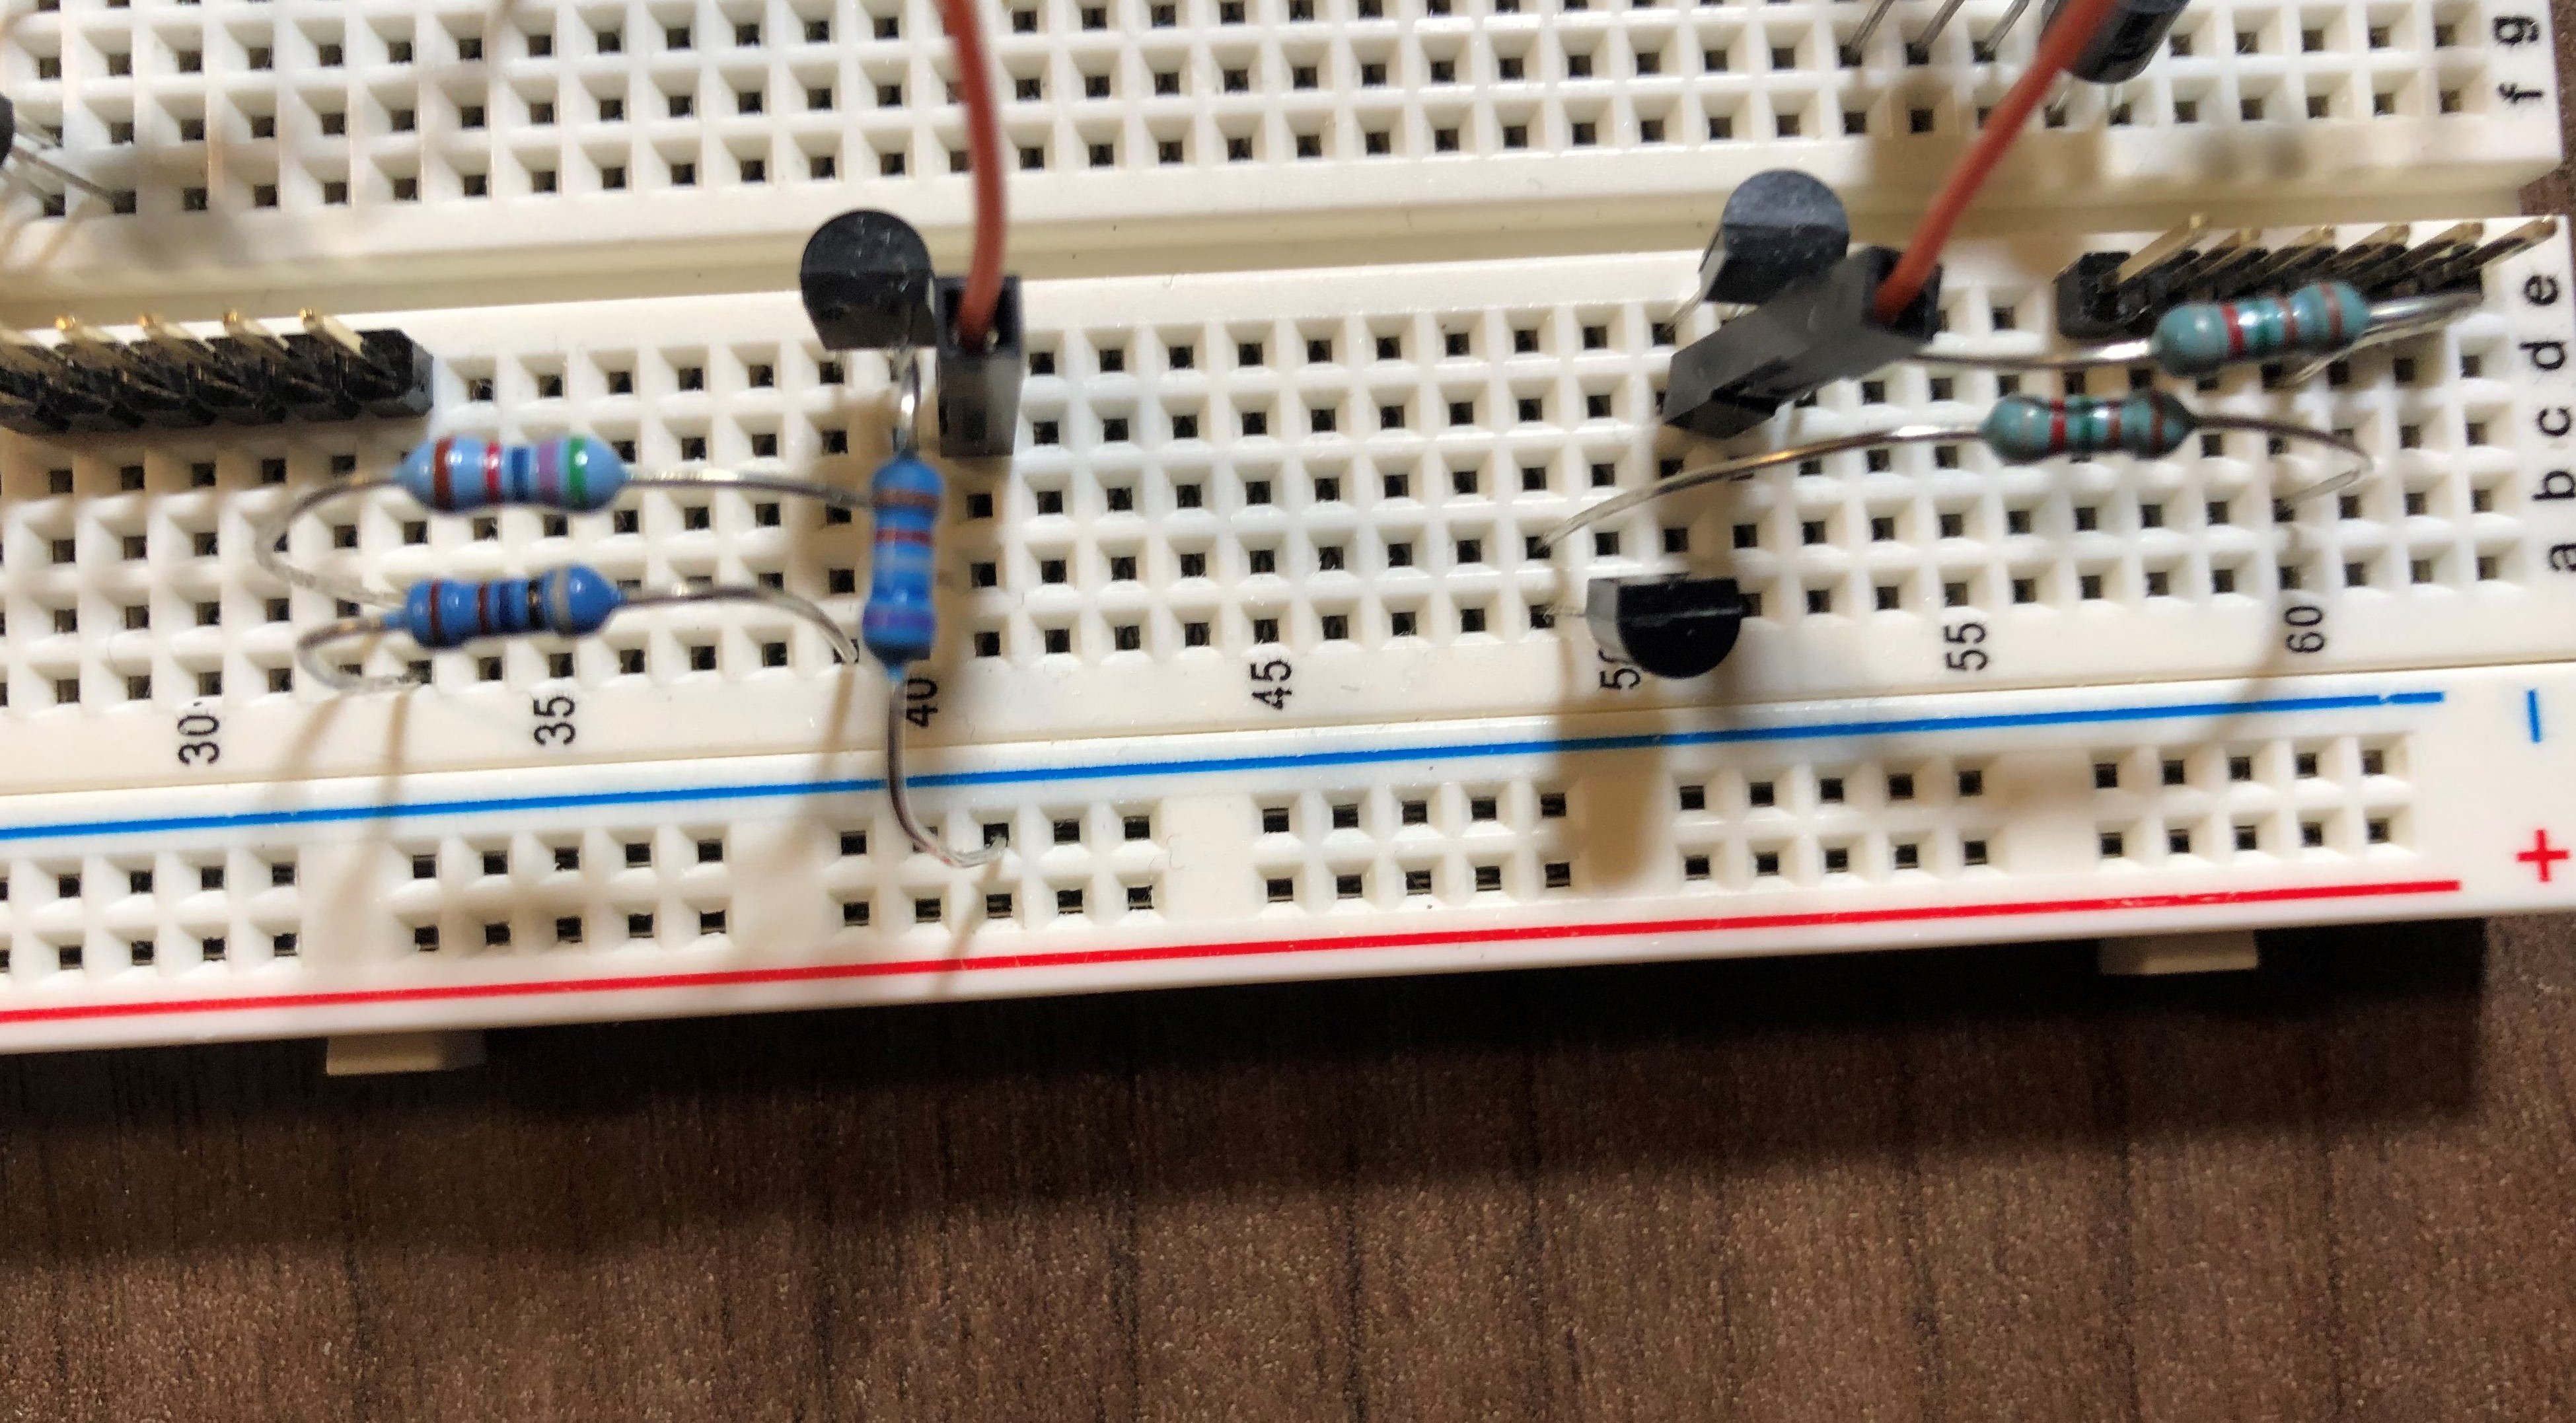
\includegraphics[width=\textwidth]{Part3B}
        \caption{Part 3: D Circuit}
    \end{subfigure}
    \caption{Circuits for Part 3}
\end{figure}
\end{document}